\documentclass[10pt]{article}
\usepackage[spanish]{babel}
\usepackage[utf8]{inputenc}
\usepackage[T1]{fontenc}
\usepackage{amsmath}
\usepackage{amsfonts}
\usepackage{amssymb}
\usepackage[version=4]{mhchem}
\usepackage{stmaryrd}
\usepackage{graphicx}
\usepackage[export]{adjustbox}
\graphicspath{ {./images/} }
\usepackage{bbold}

\begin{document}
\section*{Capítulo 5}
\section*{Programación lineal entera}
\section*{1. Introducción.}
Un problema de programación lineal entera es un problema de programación lineal con la restricción adicional de que algunas de las variables deben tomar valores enteros. Cuando todas las variables deben tomar valores enteros decimos que se trata de un problema de programación lineal entera puro, en caso contrario decimos que es mixto. Diremos que una variable es binaria si sólo puede tomar los valores 0 y 1 .\\
Una gran variedad de problemas combinatorios pueden ser planteados como problemas de programación lineal entera. Veamos algunos ejemplos.

Ejemplo 1.1. El problema de la mochila.\\
Se desea cargar en una mochila $x_{j}$ unidades del producto $j(1 \leq j \leq n)$. Supongamos que cada unidad del producto $j$ tiene asignado un peso $p_{j}$ y un valor $v_{j}$. Queremos determinar la carga de máximo valor con la condición de que el peso total de la carga de la mochila no supere un dado peso $P$, es decir, queremos resolver el problema

$$
\begin{aligned}
& \max \sum_{j} v_{j} x_{j} \\
& \sum_{j} p_{j} x_{j} \leq P \\
& x_{j} \geq 0, \quad x_{j} \text { entero }
\end{aligned}
$$

Si además agregamos la condición de que todas las variables $x_{j}$ sean binarias esto resuelve el problema de elegir un subconjunto de productos con máximo valor cuyo peso total no supere $P$.

Ejemplo 1.2. El problema de la carga fija.\\
Un centro industrial posee una usina con tres generadores. Supongamos que cada generador $i$ puede operar a niveles $x_{i}$ de $\mathrm{kw} / \mathrm{h}, 0 \leq x_{i} \leq a_{i}$ y que conocemos una función $y_{i}=y_{i}\left(x_{i}\right)$ que calcula la cantidad de kilogramos de vapor por hora consumidos en función del nivel $x_{i}$ de $\mathrm{kw} / \mathrm{h}$ al que opera el generador $i$. Supongamos además que la función $y_{i}$ es lineal en el intervalo ( $0, a_{i}$ ] y tiene una discontinuidad en el origen, donde vale cero, es decir, que

$$
y_{i}\left(x_{i}\right)= \begin{cases}c_{i} x_{i}+b_{i} & \text { si } x_{i}>0 \\ 0 & \text { si } x_{i}=0\end{cases}
$$

Esta discontinuidad se debe a que cuando el generador no está funcionando $x_{i}=0=y_{i}\left(x_{i}\right)$ pero para comenzar a funcionar necesita una cantidad fija $b_{i}$ de vapor para que se ponga en marcha la turbina.\\
Sea $C$ la cantidad de $\mathrm{kw} / \mathrm{h}$ requeridos en un momento dado. Queremos determinar cuál es el nivel $x_{i}$ al que debe operarse cada generador $i$ para producir los $\mathrm{kw} / \mathrm{h}$ requeridos de modo que la cantidad total de consumo de vapor sea mínima, es decir, queremos resolver el problema

$$
\begin{aligned}
& \min \sum_{i} y_{i}\left(x_{i}\right) \\
& x_{1}+x_{2}+x_{3}=C \\
& 0 \leq x_{i} \leq a_{i}
\end{aligned}
$$

Notemos que este no es un problema de programación lineal ya que el funcional no es una función lineal. Para resolverlo planteamos un problema auxiliar introduciendo tres variables binarias $\delta_{i}$ que valdrán 1 si el\\
generador $i$ está funcionando y 0 si no. Dejamos a cargo del lector verificar que si ( $x, \delta$ ) es una solución óptima del problema auxiliar

$$
\begin{gathered}
\min \sum_{i} c_{i} x_{i}+b_{i} \delta_{i} \\
x_{1}+x_{2}+x_{3}=C \\
0 \leq x_{i} \leq a_{i} \delta_{i} \\
0 \leq \delta_{i} \leq 1, \quad \delta_{i} \text { entero }
\end{gathered}
$$

entonces $x$ es una solución óptima del problema original.\\
Ejemplo 1.3. Condición either ... or.\\
Consideremos el problema


\begin{gather*}
\max x_{1}+x_{2} \\
5 x_{1}+2 x_{2} \leq 10 \text { o } x_{1}+2 x_{2} \leq 4  \tag{1}\\
x_{i} \geq 0
\end{gather*}


Observemos que este no es un problema de programación lineal ya que el conjunto de soluciones factibles no es convexo:\\
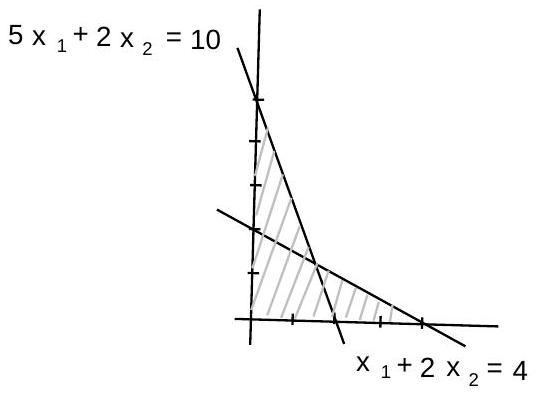
\includegraphics[max width=\textwidth, center]{2025_09_05_458e5b1ce89abceb5d44g-02}

Sin embargo, podemos convertirlo en un problema de programación lineal entera introduciendo una variable binaria $\delta$ y una constante $c$ adecuada.\\
Veamos cómo hacer esto: sea $c$ una constante que satisface

$$
\begin{aligned}
& 5 x_{1}+2 x_{2} \leq 10 \Longrightarrow x_{1}+2 x_{2} \leq 4+c \\
& x_{1}+2 x_{2} \leq 4 \Longrightarrow 5 x_{1}+2 x_{2} \leq 10+c
\end{aligned}
$$

para todo $x_{1}, x_{2} \geq 0$. Por ejemplo, en este caso podemos tomar $c=15$ ya que dados $x_{1}, x_{2} \geq 0$, si $5 x_{1}+2 x_{2} \leq 10$ entonces $x_{1} \leq 2$ y $x_{2} \leq 5$ de donde $x_{1}+2 x_{2} \leq 12 \leq 4+15$ y si $x_{1}+2 x_{2} \leq 4$ entonces $x_{1} \leq 4$ y $x_{2} \leq 2$ de donde $5 x_{1}+2 x_{2} \leq 24 \leq 10+15$.\\
Ahora consideramos el problema de programación lineal entera


\begin{gather*}
\max x_{1}+x_{2} \\
5 x_{1}+2 x_{2} \leq 10+c \delta \\
x_{1}+2 x_{2} \leq 4+c(1-\delta)  \tag{2}\\
x_{i} \geq 0 \\
0 \leq \delta \leq 1, \quad \delta \text { entero }
\end{gather*}


Si $\left(\bar{x}_{1}, \bar{x}_{2}, \delta\right)$ es una solución óptima de (2), como $\delta=0$ o 1 entonces se tiene que ( $\bar{x}_{1}, \bar{x}_{2}$ ) es una solución óptima de (1). En efecto, si $\delta=0$ entonces $5 \bar{x}_{1}+2 \bar{x}_{2} \leq 10$ y si $\delta=1$ entonces $\bar{x}_{1}+2 \bar{x}_{2} \leq 4$, de donde resulta que $\left(\bar{x}_{1}, \bar{x}_{2}\right)$ es una solución factible de (1). Veamos que es óptima. Sea ( $x_{1}, x_{2}$ ) una solución factible de (1). Por la forma en la que elegimos $c$ se tiene\\
i) si $5 x_{1}+2 x_{2} \leq 10$ entonces $x_{1}+2 x_{2} \leq 4+c$. Luego, ( $x_{1}, x_{2}, 0$ ) es una solución factible de ( 2 ) y por lo tanto $x_{1}+x_{2} \leq \bar{x}_{1}+\bar{x}_{2}$.\\
ii) si $x_{1}+2 x_{2} \leq 4$ entonces $5 x_{1}+2 x_{2} \leq 10+c$. Luego, ( $x_{1}, x_{2}, 1$ ) es una solución factible de (2) y por lo tanto $x_{1}+x_{2} \leq \bar{x}_{1}+\bar{x}_{2}$.

Ejemplo 1.4. Función objetivo no lineal.\\
Consideremos el problema

$$
\begin{gathered}
\min \sum_{j} f_{j}\left(x_{j}\right) \\
A x=b \\
x \geq 0
\end{gathered}
$$

Si fuera $f_{j}\left(x_{j}\right)=c_{j} x_{j}$ se trataría de un problema de programación lineal. Pero supongamos que las funciones $f_{j}$ sean contínuas pero no lineales. En tal caso, a cada $f_{j}$ la podemos aproximar por trozos lineales como indica el siguiente gráfico\\
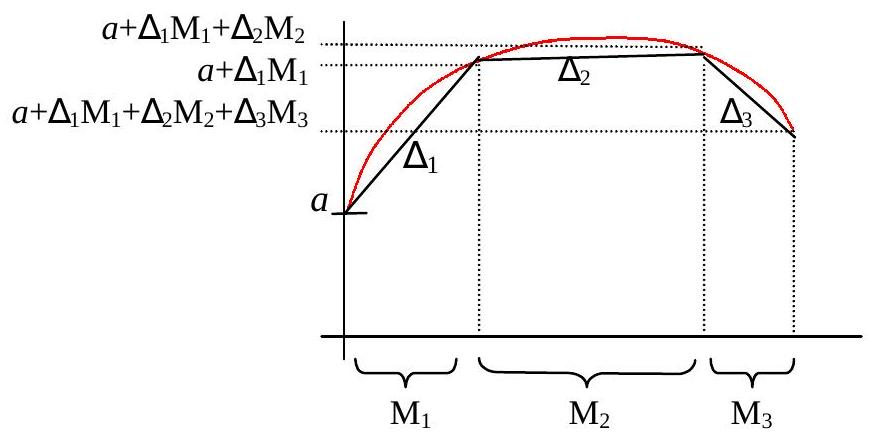
\includegraphics[max width=\textwidth, center]{2025_09_05_458e5b1ce89abceb5d44g-03}\\
donde $M_{i}>0$ y en cada trozo lineal hemos indicado su pendiente $\Delta_{i}$. Veamos cómo podemos describir esto. Hacemos el reemplazo $x_{j}=y_{1}+y_{2}+y_{3}, f_{j}=a+\Delta_{1} y_{1}+\Delta_{2} y_{2}+\Delta_{3} y_{3}$.\\
Con las restricciones

$$
\begin{gathered}
0 \leq y_{i} \leq M_{i} \\
y_{1} \geq M_{1} \delta_{1} \\
M_{2} \delta_{2} \leq y_{2} \leq M_{2} \delta_{1} \\
y_{3} \leq M_{3} \delta_{2} \\
0 \leq \delta_{i} \leq 1, \quad \delta_{i} \text { entero }
\end{gathered}
$$

resulta que

$$
\begin{aligned}
& y_{2}>0 \Longrightarrow y_{1}=M_{1} \\
& y_{3}>0 \Longrightarrow y_{2}=M_{2}
\end{aligned}
$$

Luego, como $x_{j}=y_{1}+y_{2}+y_{3}$ se tiene que\\
i) $0 \leq x_{j} \leq M_{1} \Longleftrightarrow y_{2}=0=y_{3}$\\
ii) $M_{1}<x_{j} \leq M_{1}+M_{2} \Longleftrightarrow y_{2}>0, y_{3}=0$\\
iii) $M_{1}+M_{2}<x_{j} \leq M_{1}+M_{2}+M_{3} \Longleftrightarrow y_{3}>0$

En efecto,\\
i) Supongamos que $0 \leq x_{j} \leq M_{1}$. Si fuese $y_{2}>0$ entonces $y_{1}=M_{1}$ de donde $x_{j}=M_{1}+y_{2}+y_{3}>M_{1}$. Luego debe ser $y_{2}=0$. Pero entonces debe ser $y_{3}=0$ ya que si $y_{3}>0$ entonces $y_{2}=M_{2}>0$. Recíprocamente, si $y_{2}=0=y_{3}$ entonces $x_{j}=y_{1}$ y como $0 \leq y_{1} \leq M_{1}$ entonces $0 \leq x_{j} \leq M_{1}$.\\
ii) Supongamos que $M_{1}<x_{j} \leq M_{1}+M_{2}$. Si fuese $y_{3}>0$ entonces $y_{2}>M_{2}>0$ y por lo tanto $y_{1}=M_{1}$. Pero entonces $x_{j}=M_{1}+M_{2}+y_{3}>M_{1}+M_{2}$. Luego debe ser $y_{3}=0$ y, por i), también debe ser $y_{2}>0$. Recíprocamente, si $y_{2}>0$ e $y_{3}=0$ entonces $y_{1}=M_{1}$, de donde $x_{j}=M_{1}+y_{2}$ y como $0<y_{2} \leq M_{2}$ entonces $M_{1}<x_{j} \leq M_{1}+M_{2}$.\\
Dejamos al lector la tarea de verificar la validez de iii).\\
Esto implica que para $x_{j}$ tal que $0 \leq x_{j} \leq M_{1}$ estamos reemplazando $x_{j}$ por $y_{1}$ y $f_{j}$ por $a+\Delta_{1} y_{1}$, es decir, por el primer trozo lineal, para $x_{j}$ tal que $M_{1}<x_{j} \leq M_{1}+M_{2}$ estamos reemplazando $x_{j}$ por $M_{1}+y_{2}$ con $0<y_{2} \leq M_{2}$ y $f_{j}$ por $a+\Delta_{1} M_{1}+\Delta_{2} y_{2}$, es decir, por el segundo trozo lineal y, para $x_{j}$ tal que $M_{1}+M_{2}<x_{j} \leq M_{1}+M_{2}+M_{3}$ estamos reemplazando $x_{j}$ por $M_{1}+M_{2}+y_{3}$ con $0<y_{3} \leq M_{3}$ y $f_{j}$ por $a+\Delta_{1} M_{1}+\Delta_{2} M_{2}+\Delta_{3} y_{3}$, es decir, por el tercer trozo lineal.

Ejemplo 1.5. Variables discretas.\\
Supongamos que en un problema de programación lineal queremos agregar la restricción de que una variable $x$ sólo pueda tomar un número finito de valores $a_{1}, \ldots, a_{k}$. Esto se puede describir mediante la introducción de $k$ variables binarias $\delta_{1}, \ldots, \delta_{k}$ y reemplazando $x$ por $a_{1} \delta_{1}+\cdots+a_{k} \delta_{k}$ con las restricciones

$$
\begin{gathered}
\delta_{1}+\cdots+\delta_{k}=1 \\
0 \leq \delta_{i} \leq 1 \quad \delta_{i} \text { entero }
\end{gathered}
$$

Ejemplo 1.6. Cutting-stock problem.\\
La máquina de casting produce bobinas de celofán de 200 pulgadas de ancho. Los clientes realizan pedidos por bobinas de anchos menores. Sean $w_{1}, \ldots, w_{m}$ los posibles anchos pedidos por los clientes. Llamaremos pattern a cualquier sucesión de enteros no negativos $\left(a_{1}, \ldots, a_{m}\right)$ tal que $a_{1} w_{1}+\cdots+a_{m} w_{m} \leq 200$, con la que luego se instruye al operario para que corte la bobina original de 200 pulgadas para que resulten $a_{i}$ bobinas de ancho $w_{i}(1 \leq i \leq m)$. La siguiente figura muestra una bobina con el pattern de corte $(4,2,1)$ para los anchos $w_{1}=20, w_{2}=30$ y $w_{3}=40$.\\
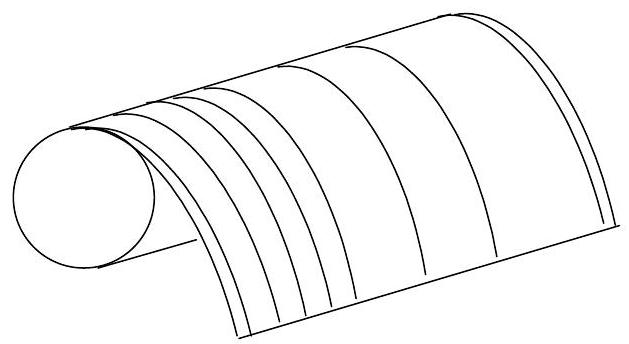
\includegraphics[max width=\textwidth, center]{2025_09_05_458e5b1ce89abceb5d44g-04}

En este caso queda un borde de 10 pulgadas de descarte a cada lado.\\
El problema consiste en satisfacer los pedidos utilizando un mínimo número de bobinas. Sea $b_{i}$ el número de bobinas de ancho $w_{i}$ pedidas por los clientes ( $1 \leq i \leq m$ ).\\
Notemos que el conjunto de patterns $\left\{\left(a_{1}, \ldots, a_{m}\right\} / a_{1} w_{1}+\cdots+a_{m} w_{m} \leq 200\right\}$ es finito. Sean $p_{1}, \ldots, p_{n}$ sus elementos. Para cada $j$ denotemos por $a_{1 j}, \ldots, a_{m j}$ a los enteros no negativos tales que $p_{j}=\left(a_{1 j}, \ldots, a_{m j}\right)$ y $a_{1 j} w_{1}+\cdots+a_{m j} w_{m} \leq 200$. Sea $x_{j}$ la cantidad de bobinas de 200 pulgadas de ancho que se cortan según el $j$-ésimo pattern $(1 \leq j \leq n)$. Entonces el problema se puede plantear en la forma

$$
\begin{aligned}
& \min \sum_{j} x_{j} \\
& \sum_{j} a_{i j} x_{j} \geq b_{i} \\
& \quad x_{j} \geq 0 \quad x_{j} \text { entero }
\end{aligned}
$$

En la práctica este problema no puede resolverse con la condición de que los valores de $x_{j}$ sean enteros porque el número de columnas de la matriz $A=\left\|a_{i j}\right\|$ es enorme (la cantidad $n$ de patterns es el cardinal del conjunto de $m$-uplas $\left(a_{1}, \ldots, a_{m}\right)$ tales que $\sum a_{i} w_{i} \leq 200$ ). Lo que se hace, en general, es resolver el problema sin la restricción de que $x_{j}$ sea entero y luego se redondea el resultado. Aún así no es fácil hallar la solución cuando $n$ es muy grande. En ese caso se procede de la siguiente manera:\\
Como el problema que queremos resolver es


\begin{gather*}
\min \sum_{j} x_{j} \\
\sum_{j} a_{i j} x_{j} \geq b_{i}  \tag{3}\\
x_{j} \geq 0
\end{gather*}


que puede escribirse, agregando las correspondientes variables de holgura, en la forma

$$
\begin{aligned}
& \min \sum_{j} x_{j}+0 s_{1}+\cdots+0 s_{m} \\
& \sum_{j} a_{i j} x_{j}-s_{i}=b_{i} \\
& \quad x_{j}, s_{i} \geq 0
\end{aligned}
$$

es decir, en la forma

$$
\begin{aligned}
& \min \sum_{j} x_{j}+0 s_{1}+\cdots+0 s_{m} \\
& \left(\begin{array}{ll}
A & -I
\end{array}\right)\binom{x}{s}=b \\
& \quad x, s \geq 0
\end{aligned}
$$

entonces el problema dual de (3) resulta ser

$$
\begin{gathered}
\max y b \\
y \cdot\left(\begin{array}{ll}
A & -I
\end{array}\right) \leq(\underbrace{1, \ldots, 1}_{n}, \underbrace{0, \ldots, 0}_{m})
\end{gathered}
$$

es decir,


\begin{align*}
& \max y b \\
& y \cdot A_{j} \leq 1  \tag{4}\\
& -y \leq 0
\end{align*}


donde $A_{j}$ es la $j$-ésima columna de $A$. Además, las condiciones de holgura complementaria son

$$
\begin{aligned}
\left(1-y \cdot A_{j}\right) \cdot x_{j}=0 & (1 \leq j \leq n) \\
-y_{i} \cdot s_{i}=0 & (1 \leq i \leq m)
\end{aligned}
$$

Luego, si $x$ es una solución óptima del problema primal e $y$ es el correspondiente óptimo del dual, entonces $y \geq 0$ e $y . A_{j} \leq 1$. Además, si $x$ e $y$ son soluciones de los problemas primal y dual respectivamente, y satisfacen las condiciones de holgura complementaria entonces son óptimos.\\
Supongamos que hemos resuelto el problema utilizando en lugar de la matriz $A$ la submatriz formada por un subconjunto relativamente pequeño $\left\{A_{j_{1}}, \ldots, A_{j_{r}}\right\}$ de columnas de $A$ obteniendo una solución óptima $\left(u_{j_{1}}, \ldots, u_{j_{r}}\right)$ y que $v=\left(v_{1}, \ldots, v_{m}\right)$ es el correspondiente óptimo del dual de este nuevo problema.

Luego $v \geq 0$ y satisface $v . A_{j_{t}} \leq 1$ para $t=1, \ldots, r$.\\
Si fuese v. $A_{j} \leq 1$ para todo $1 \leq j \leq n$ entonces $v$ sería una solución factible de (4). Además, como $u_{j_{t}} \geq 0$ para $t=1, \ldots, r$ y se verifica $a_{i j_{1}} u_{j_{1}}+\cdots+a_{i j_{r}} u_{j_{r}} \geq b_{i}$ para $i=1, \ldots, m$, tomando $u_{j}=0$ para $j \neq j_{1}, \ldots, j_{r}$ resulta que $u=\left(u_{1}, \ldots, u_{n}\right)$ es una solución factible de (3). Como además $v$ y ( $u_{j_{1}}, \ldots, u_{j_{r}}$ ) satisfacen las condiciones de holgura complementaria del problema con reducción de columnas entonces verifican

$$
\begin{array}{rr}
\left(1-y \cdot A_{j_{t}}\right) \cdot u_{j_{t}}=0 & (1 \leq t \leq r) \\
-y_{i} \cdot s_{i}=0 & (1 \leq i \leq m)
\end{array}
$$

de donde resulta que $u$ y $v$ satisfacen las condiciones de holgura complementaria del problema original. Luego $u$ es una solución óptima de (3).\\
Veamos cómo determinar si $v . A_{j} \leq 1$ para todo $1 \leq j \leq n$ y qué hacer si esto no se satisface.\\
En primer lugar, resolvemos el problema de la mochila


\begin{align*}
& \max \sum_{i} v_{i} z_{i} \\
& \sum_{i} w_{i} z_{i} \leq 200  \tag{5}\\
& z_{i} \geq 0 \quad z_{i} \text { entero }
\end{align*}


Si el óptimo $\left(\bar{z}_{1}, \ldots, \bar{z}_{m}\right)$ de (5) satisface $\sum v_{i} \bar{z}_{i} \leq 1$, todos los patterns ( $a_{1 j}, \ldots, a_{m j}$ ) satisfacen $\sum v_{i} a_{i j} \leq 1$, es decir, v. $A_{j} \leq 1$ para todo $j$ como queríamos (notar que todo pattern es una solución factible de (5)). En caso contrario, al terminar el algoritmo para el problema reducido que utiliza, en lugar de la matriz $A$, la submatriz formada por las columnas $A_{j_{1}}, \ldots, A_{j_{r}}$ de $A$, lo continuamos, ahora incorporando la columna

$$
\left(\begin{array}{c}
1 \\
\bar{z}_{1} \\
\vdots \\
\bar{z}_{m}
\end{array}\right)
$$

(ver capítulo 1 , sección 10: utilizando el algoritmo simplex revisado es posible incorporar una columna en cualquier momento). Como $\left(\bar{z}_{1}, \ldots, \bar{z}_{m}\right)$ es una solución factible de (5) entonces es un pattern y por lo tanto alguna de las columnas de $A$, y como estamos suponiendo que $\sum v_{i} \bar{z}_{i}>1$ entonces no es ninguna de las columnas $j_{1}, \ldots, j_{r}$. Luego, al continuar el algoritmo incorporando esta columna lo que estamos haciendo es repetir el proceso anterior, ahora para un problema reducido que utiliza $r+1$ columnas de $A$. Repetimos este procedimiento hasta que el óptimo $v$ correspondiente al óptimo del problema reducido verifique $v . A_{j} \leq 1$ para todo $1 \leq j \leq n$.

Ejemplo 1.7. Job scheduling.\\
Los tubos de acero se elaboran en cuatro etapas sucesivas: laminación, ajuste, tratamiento térmico y roscado. Se agrupan en lotes, cada uno conteniendo todos los tubos con una misma especificación técnica. Cada lote pasa por las cuatro etapas y, en cada etapa, el orden de procesamiento de los lotes no tiene porqué coincidir. Además, entre dos etapas puede haber un stock intermedio.\\
Supongamos que hay $n$ lotes y sea $p_{i k}(1 \leq i \leq n, \quad 1 \leq k \leq 4)$ el tiempo de procesamiento del lote $i$ en la etapa $k$. Supongamos además que el procesamiento se inicia en el instante cero y sea $z$ el instante en que se terminan de procesar todos los lotes. Se desea determinar en qué instante $x_{i k}$ se debe iniciar el proceso del lote $i$ en la etapa $k(1 \leq i \leq n, \quad 1 \leq k \leq 4)$ de manera tal que el valor de $z$ sea mínimo. Las restricciones a tener en cuenta son:\\
i) el procesamiento de un lote no puede iniciarse en una etapa si no ha sido terminado su procesamiento en la etapa anterior.\\
ii) dos lotes no pueden procesarse simultáneamente en una misma etapa, es decir, para cada par de lotes $i \neq j$, el lote $i$ debe haber salido de la etapa $k$ antes de que entre en ella el lote $j$ o viceversa.

Luego, el problema puede plantearse en la forma

$$
\begin{gathered}
\min z \\
x_{i 1}+p_{i 1} \leq x_{i 2} \\
x_{i 2}+p_{i 2} \leq x_{i 3} \\
x_{i 3}+p_{i 3} \leq x_{i 4} \\
x_{i 4}+p_{i 4} \leq z \\
x_{i k}+p_{i k} \leq x_{j k} \text { o } x_{j k}+p_{j k} \leq x_{i k} \quad(i \neq j) \\
x_{i k} \geq 0
\end{gathered}
$$

Notemos que es la condición

$$
x_{i k}+p_{i k} \leq x_{j k} \text { o } x_{j k}+p_{j k} \leq x_{i k} \quad(i \neq j)
$$

la que hace que este sea un problema de programación lineal entera. Históricamente, el planteo del problema de scheduling llamó la atención por la simplicidad de su solución en el caso en que haya dos etapas (ver [Jo, 1954]).\\
No se ha encontrado una solución simple para tres o más etapas. En el caso de dos o tres etapas la solución óptima tiene la particularidad de que el orden de procesamiento de los lotes es el mismo en todas las etapas.

Ejemplo 1.8. El problema de los cuatro colores.\\
Supongamos que queremos pintar las distintas regiones de un mapa que está dibujado sobre un plano de manera tal que regiones adyacentes estén pintadas de colores distintos. La siguiente figura muestra un ejemplo donde se necesitan cuatro colores.\\
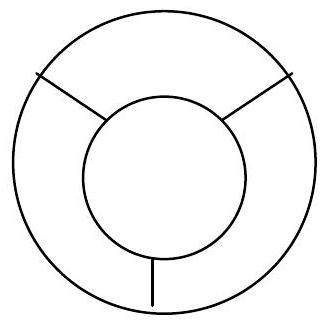
\includegraphics[max width=\textwidth, center]{2025_09_05_458e5b1ce89abceb5d44g-07}

Durante 150 años se conjeturó que cualquier mapa se podía pintar, con la mencionada restricción, con a lo sumo cuatro colores. El esfuerzo hecho para resolver el problema fue uno de los principales motivos del desarrollo de la teoría de grafos. Finalmente, en 1976 se demostró esta conjetura (ver [Ap-Ha, 1978]).\\
Sea $G=(V, E)$ un grafo no dirigido. Colorear el grafo significa asignar un color a cada vértice $i$ de manera tal que $i$ y $j$ tengan colores distintos para toda rama $(i, j) \in E$.\\
El mínimo número de colores necesarios para colorear a $G$ se llama el número cromático de $G$.\\
Todo mapa se puede representar en un grafo planar no dirigido (para la definición de grafo planar ver sección 3 del capítulo 4) donde cada vértice representa una región del mapa y dos vértices están unidos por una rama si y sólo si las regiones que representan son adyacentes. El teorema de los cuatro colores afirma que el número cromático de cualquier grafo planar es a lo sumo cuatro.\\
Supongamos ahora que tenemos un grafo no dirigido cualquiera (no necesariamente planar) y queremos ver si podemos colorearlo con a lo sumo cuatro colores. Sean $0,1,2,3$ los cuatro colores. Entonces estos colores\\
son suficientes si y sólo si para cada vértice $i$ existe $x_{i} \in\{0,1,2,3\}$ (el color asignado al vértice $i$ ) tal que $x_{i} \neq x_{j}$ para todo $(i, j) \in E$.\\
Observando que $x_{i} \neq x_{j}$ si y sólo si $x_{i}>x_{j}$ o $x_{j}>x_{i}$ si y sólo si $1 \leq x_{i}-x_{j}$ o $1 \leq x_{j}-x_{i}$, el problema se traduce en determinar si


\begin{gather*}
1 \leq x_{i}-x_{j} \text { o } 1 \leq x_{j}-x_{i} \quad((i, j) \in E)  \tag{6}\\
0 \leq x_{i} \leq 3, \quad x_{i} \text { entero }
\end{gather*}


es factible. Sean $s_{i j}, t_{i j}((i, j) \in E)$ nuevas variables y consideremos el problema


\begin{gather*}
\min z \\
z=\sum_{(i, j) \in E} s_{i j}+t_{i j} \\
1 \leq x_{i}-x_{j}+s_{i j} \text { o } 1 \leq x_{j}-x_{i}+t_{i j} \quad((i, j) \in E)  \tag{7}\\
s_{i j}, t_{i j} \geq 0 \\
0 \leq x_{i} \leq 3, \quad x_{i} \text { entero }
\end{gather*}


Entonces (6) es factible si y sólo si (7) tiene una solución óptima tal que $z=0$.\\
Ejemplo 1.9. El problema del viajante.\\
Un viajante debe visitar las ciudades $1,2, \ldots, n$ partiendo de la ciudad 0 , pasando por cada una de las ciudades $1,2, \ldots, n$ una y sólo una vez y volviendo luego a la ciudad 0 . Sea $c_{i j}$ el costo de viajar de la ciudad $i$ a la ciudad $j(0 \leq i, j \leq n)$. Si no hay camino de $i$ a $j$ tomamos $c_{i j}=\infty$.\\
A cada una de las posibles maneras de hacer el recorrido la llamamos un circuito Hamiltoniano. Definimos el costo de un tal circuito como la suma de los costos de los tramos que lo componen. El problema consiste en hallar un circuito Hamiltoniano de mínimo costo.\\
Representamos la situación en un grafo dirigido completo $G=(V, E)$ donde

$$
V=\{0,1,2, \ldots, n\}
$$

y asignamos $\operatorname{costo~} c_{i j}$ a cada rama $(i, j)$.\\
Dado un circuito Hamiltoniano $\mathcal{C}$ (es decir, un circuito dirigido en $G$ que pasa por cada vértice una y sólo una vez), para cada $(i, j)$ sea

$$
\delta_{i j}= \begin{cases}1 & \text { si }(i, j) \in \mathcal{C} \\ 0 & \text { si no }\end{cases}
$$

Entonces el costo de $\mathcal{C}$ es $\sum c_{i j} \delta_{i j}$.\\
Observemos que para cada vértice $i$ hay una sola rama de $\mathcal{C}$ cuya cola es $i$ y una sola rama de $\mathcal{C}$ cuya punta es $i$. Luego se satisface

\[
\begin{array}{ll}
\sum_{j} \delta_{i j}=1 & (0 \leq i \leq n) \\
\sum_{i} \delta_{i j}=1 & (0 \leq j \leq n) \tag{8}
\end{array}
\]

Supongamos ahora que para cada $(i, j)$ tenemos definido un $\delta_{i j}$ tal que $\delta_{i j}=0$ o $\delta_{i j}=1$ y de manera tal que valga (8).\\
Si el conjunto de ramas $(i, j)$ tales que $\delta_{i j}=1$ fuese un circuito entonces podríamos pensar a cada circuito Hamiltoniano como una solución factible de

\[
\begin{array}{ll}
\sum_{j} \delta_{i j}=1 & (0 \leq i \leq n) \\
\sum_{i} \delta_{i j}=1 & (0 \leq j \leq n)  \tag{9}\\
0 \leq \delta_{i j} \leq 1, & \delta_{i j} \text { entero }
\end{array}
\]

cuyo costo es $\sum c_{i j} \delta_{i j}$. Lamentablemente esto no es así, como lo muestra el siguiente ejemplo. Sea $V=\{0,1,2,3,4,5\}$ y tomemos

$$
\delta_{01}=\delta_{20}=\delta_{12}=\delta_{34}=\delta_{45}=\delta_{53}=1
$$

y los restantes $\delta_{i j}$ iguales a cero. Es decir, el conjunto $(i, j)$ tales que $\delta_{i j}=1$ es

$$
\{(0,1),(2,0),(1,2),(3,4),(4,5),(5,3)\}
$$

En este caso $\delta_{i j}(0 \leq i, j \leq 5)$ es una solución factible de (9) pero el conjunto de ramas $(i, j)$ tales que $\delta_{i j}=1$ no forman un circuito sino dos subcircuitos:\\
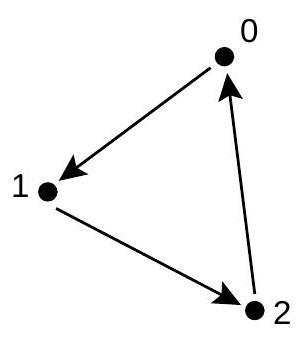
\includegraphics[max width=\textwidth, center]{2025_09_05_458e5b1ce89abceb5d44g-09(1)}\\
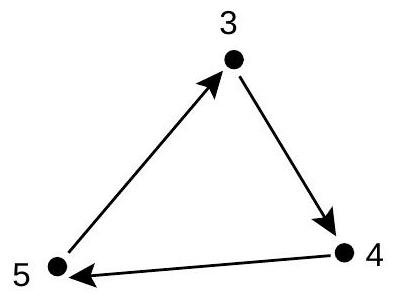
\includegraphics[max width=\textwidth, center]{2025_09_05_458e5b1ce89abceb5d44g-09}

Pero agregando la ingeniosa condición

$$
u_{i}-u_{j}+n \delta_{i j} \leq n-1 \quad(1 \leq i, j \leq n, i \neq j)
$$

donde $u_{i}(1 \leq i \leq n)$ son números reales nos permitirá plantear el problema del viajante por programación lineal entera. Esto se debe a que si $\delta_{i j}$ es una solución factible de (9) entonces existen $u_{i}$ satisfaciendo esta nueva condición si y sólo si el conjunto de ramas $(i, j)$ tales que $\delta_{i j}=1$ es un circuito. En tal caso el costo de ese circuito es $\sum c_{i j} \delta i j$.

Afirmación. El problema de programación lineal entera


\begin{align*}
\min \sum c_{i j} \delta_{i j} & \\
\sum_{j} \delta_{i j}=1 & (0 \leq i \leq n) \\
\sum_{i} \delta_{i j}=1 & (0 \leq j \leq n)  \tag{10}\\
u_{i}-u_{j}+n \delta_{i j} \leq n-1 & (1 \leq i, j \leq n, i \neq j) \\
0 \leq \delta_{i j} \leq 1, & \delta_{i j} \text { entero }
\end{align*}


resuelve el problema del viajante.\\
Demostración: Mostraremos que cada circuito Hamiltoniano puede representarse como una solución factible de (10).\\
Supongamos que $\mathcal{C}$ es un circuito Hamiltoniano. Para cada $(i, j)$ sea

$$
\delta_{i j}= \begin{cases}1 & \text { si }(i, j) \in \mathcal{C} \\ 0 & \text { si no }\end{cases}
$$

Sea $u_{i}=1$ si $i$ es la primera ciudad visitada, $u_{i}=2$ si $i$ es la segunda ciudad visitada, etc. Por ejemplo, si $n=5$ y el circuito es

$$
0 \longrightarrow 2 \longrightarrow 5 \longrightarrow 3 \longrightarrow 1 \longrightarrow 4 \longrightarrow 0
$$

entonces

$$
u_{1}=4, \quad u_{2}=1, \quad u_{3}=3, \quad u_{4}=5, \quad u_{5}=2
$$

Entonces

$$
u_{i}-u_{j}+n \delta_{i j}= \begin{cases}u_{i}-u_{j} & \text { si }(i, j) \notin \mathcal{C} \\ -1+n & \text { si }(i, j) \in \mathcal{C}\end{cases}
$$

ya que si $(i, j) \notin \mathcal{C}$ entonces $\delta_{i j}=0$ y si $(i, j) \in \mathcal{C}$ entonces el viajante visita $j$ justo después de visitar $i$, de donde $u_{j}=u_{i}+1$ y como $(i, j) \in \mathcal{C}$ entonces $\delta_{i j}=1$.\\
Luego, como $1 \leq u_{i} \leq n$ entonces $u_{i}-u_{j}+n \delta_{i j} \leq n-1$ para todo $i \neq j(1 \leq i, j \leq n)$. Esto muestra que cada circuito Hamiltoniano determina una solución factible de (10).\\
Recíprocamente, supongamos ahora que tenemos una solución factible de (10). Probaremos que el conjunto de ramas $\mathcal{C}=\left\{(i, j) / \delta_{i j}=1\right\}$ es un circuito Hamiltoniano. Como cada $\delta_{i j}$ es cero o uno y valen

$$
\begin{array}{ll}
\sum_{j} \delta_{i j}=1 & (0 \leq i \leq n) \\
\sum_{i} \delta_{i j}=1 & (0 \leq j \leq n)
\end{array}
$$

entonces para cada $i$ hay un único $j$ tal que $\delta_{i j}=1$ y un único $j$ tal que $\delta_{j i}=1$ (notemos que la segunda igualdad puede escribirse $\sum_{j} \delta_{j i}=1$ para $0 \leq i \leq n$ ). Esto significa que para cada vértice $i$ hay una sola rama de $\mathcal{C}$ cuya cola es $i$ y una sola rama de $\mathcal{C}$ cuya punta es $i$. Luego, sólo debemos ver que las ramas de $\mathcal{C}$ forman un circuito y no dos o más subcircuitos. Supongamos que formaran dos o más subcircuitos. Entonces podemos elegir uno de ellos que no pase por el vértice 0 . Sea $\mathcal{E}$ el conjunto de ramas que lo forman y sea $k=\# \mathcal{E}$. Como $u_{i}-u_{j}+n \delta_{i j} \leq n-1$ para todo $1 \leq i, j \leq n$ tal que $i \neq j$ entonces

$$
\sum_{(i, j) \in \mathcal{E}} u_{i}-u_{j}+n \delta_{i j} \leq k(n-1)
$$

Pero como para cada $i$ hay una única rama en $\mathcal{E}$ cuya cola es $i$ y una única rama cuya punta es $i$ entonces

$$
\sum_{(i, j) \in \mathcal{E}} u_{i}-u_{j}=0
$$

ya que cada $u_{i}$ aparece una vez sumando y una vez restando. Además, como las ramas de $\mathcal{E}$ forman un subcircuito de $\mathcal{C}$ entonces $\delta_{i j}=1$ para todo $(i, j) \in \mathcal{E}$. Por lo tanto,

$$
\sum_{(i, j) \in \mathcal{E}} n \delta_{i j}=k n
$$

de donde

$$
\begin{aligned}
& k n=0+k n=\sum_{(i, j) \in \mathcal{E}} u_{i}-u_{j}+\sum_{(i, j) \in \mathcal{E}} n \delta_{i j}= \\
& =\sum_{(i, j) \in \mathcal{E}} u_{i}-u_{j}+n \delta_{i j} \leq k(n-1)
\end{aligned}
$$

con lo cual se tiene que $k n \leq k(n-1)$, lo que es un absurdo pues $k>0$. Luego, cada solución factible de (10) determina un circuito Hamiltoniano. ㅁ

Ejemplo 1.10. Cuadrados latinos ortogonales.\\
Supongamos que queremos comparar el rendimiento de $n$ variedades de trigo. Si plantamos cada variedad en una franja del terreno podría ocurrir que el trigo plantado en la primera franja tuviera un alto rendimiento\\
debido a que esa zona del terreno es más fértil que las otras y no porque esa variedad de trigo sea en realidad la de mayor rendimiento. Para evitar que las diferencias en la fertilidad del suelo influyan en los resultados de nuestro experimento, conviene dividir el terreno en $n^{2}$ parcelas y plantar cada una de las $n$ variedades de trigo en $n$ parcelas de manera que cada franja (horizontal o vertical) del terreno contenga las $n$ variedades. Por ejemplo, para $n=3$, las variedades $a, b$ y $c$ podrían disponerse en la forma

\begin{center}
\begin{tabular}{|c|c|c|}
\hline
$a$ & $b$ & $c$ \\
\hline
$b$ & $c$ & $a$ \\
\hline
$c$ & $a$ & $b$ \\
\hline
\end{tabular}
\end{center}

Un cuadrado latino de $n \times n$ es una disposición de $n$ símbolos en una matriz de $n \times n$ de manera tal que cada símbolo aparezca exactamente una vez en cada fila y en cada columna.\\
El nombre de cuadrado latino tiene se debe a que Euler utilizaba como símbolos las letras $a, b, c \ldots$\\
Es fácil ver que para cualquier $n$ siempre existe un cuadrado latino de $n \times n$. En efecto, basta tomar la disposición

$$
\left(\begin{array}{cccccc}
1 & 2 & 3 & \ldots & n-1 & n \\
2 & 3 & 4 & \ldots & n & 1 \\
3 & 4 & 5 & \ldots & 1 & 2 \\
\vdots & \vdots & \vdots & \vdots & \vdots & \vdots \\
n-2 & n-1 & n & \ldots & n-4 & n-3 \\
n-1 & n & 1 & \ldots & n-3 & n-2 \\
n & 1 & 2 & \ldots & n-2 & n-1
\end{array}\right)
$$

Supongamos ahora que queremos estudiar el comportamiento de las tres variedades de trigo $a, b, c$ cuando se les aplica cada uno de los fertilizantes $\alpha, \beta, \gamma$. Para que nuestro experimento no se vea afectado por las posibles variaciones en la fertilidad del suelo, debemos disponer cada uno de los 9 pares (variedad de trigo, fertilizante) en las 9 parcelas de manera en cada fila y en cada columna aparezcan todas las variedades de trigo y todos los fertilizantes, es decir, de manera que tanto las primeras coordenadas como las segundas formen un cuadrado latino.\\
Si $A=\left\|a_{i j}\right\|$ y $B=\left\|b_{i j}\right\|$ son dos cuadrados latinos de $n \times n$, la matriz de $n \times n$ cuyo coeficiente en el lugar $i j$ es el par $\left(a_{i j}, b_{i j}\right)$ se llama la superposición de $A$ con $B$. Por lo tanto, lo que necesitamos es construír dos cuadrados latinos (uno para las variedades de trigo y otro para los fertilizantes) de forma tal que la superposición de ambos contenga todos los posibles pares (variedad de trigo, fertilizante). Por ejemplo, si consideramos los cuadrados latinos

\begin{center}
\begin{tabular}{|c|c|c|}
\hline
$a$ & $b$ & $c$ \\
\hline
$b$ & $c$ & $a$ \\
\hline
$c$ & $a$ & $b$ \\
\hline
\end{tabular}
\end{center}

\begin{center}
\begin{tabular}{|l|l|l|}
\hline
$\beta$ & $\gamma$ & $\alpha$ \\
\hline
$\alpha$ & $\beta$ & $\gamma$ \\
\hline
$\gamma$ & $\alpha$ & $\beta$ \\
\hline
\end{tabular}
\end{center}

vemos que su superposición contiene todos los posibles pares (variedad de trigo, fertilizante)

\begin{center}
\begin{tabular}{|l|l|l|}
\hline
$(a, \beta)$ & $(b, \gamma)$ & $(c, \alpha)$ \\
\hline
$(b, \alpha)$ & $(c, \beta)$ & $(a, \gamma)$ \\
\hline
$(c, \gamma)$ & $(a, \alpha)$ & $(b, \beta)$ \\
\hline
\end{tabular}
\end{center}

Esto motiva la siguiente definición:\\
Dos cuadrados latinos de $n \times n$ se dicen ortogonales (o grecolatinos) si los coeficientes de su superposición son $n^{2}$ pares distintos. En general, $m$ cuadrados latinos $L_{1}, \ldots, L_{m}$ de $n \times n$ se dicen ortogonales si $L_{i}$ y $L_{j}$ son ortogonales para todo $i \neq j(1 \leq i, j \leq m)$.\\
Euler conjeturó que no existen pares de cuadrados latinos ortogonales de $n \times n$, para $n$ de la forma $4 k+2 (k \in \mathbb{N})$. Recién en 1960 se pudo determinar que esta conjetura era falsa cuando Bose, Parker y Shrikhande probaron que, salvo para $n=2$ o 6 , siempre existe un par de cuadrados latinos ortogonales de $n \times n$.

Se puede demostrar que para todo $n \geq 2$ hay a lo sumo $n-1$ cuadrados latinos ortogonales de $n \times n$. Si para un dado $n$ hay exactamente $n-1$ cuadrados latinos ortogonales decimos que para $n$ hay un sistema completo. Se sabe que para los $n$ que son potencias de primos siempre hay un sistema completo pero, en general, para aquellos $n$ que no son potencia de un primo (salvo para algunos casos particulares) no se sabe aún si hay o no un sistema completo.\\
A continuación daremos un planteo por programación lineal entera para resolver el problema de determinar, para un $n$ dado, un par de cuadrados latinos ortogonales de $n \times n$.\\
Supongamos que tenemos dos cuadrados latinos ortogonales $A=\left\|a_{i j}\right\|, B=\left\|b_{i j}\right\|$. Entonces su superposición es la matriz $C$ cuyo coeficiente en el lugar $i j$ es el par ( $a_{i j}, b_{i j}$ ). Sin pérdida de generalidad podemos suponer que $a_{i j}, b_{i j} \in\{1,2, \ldots, n\}$.

Para cada $i, j, k, s(1 \leq i, j, k, s \leq n)$ sea $\delta_{i j k s}= \begin{cases}1 & \text { si } a_{i j}=k \text { y } b_{i j}=s \\ 0 & \text { si no }\end{cases}$\\
Como $A$ y $B$ son cuadrados latinos entonces cada $k$ aparece en una única fila y en una única columna de $A$ y cada $s$ aparece en una única fila y en una única columna de $B$. Luego se verifican las condiciones

\begin{enumerate}
  \item para cada $i, j$ existen únicos $k, s$ tales que $\delta_{i j k s}=1$.
  \item para cada $i, k$ existen únicos $j, s$ tales que $\delta_{i j k s}=1$.
  \item para cada $i, s$ existen únicos $j, k$ tales que $\delta_{i j k s}=1$.
  \item para cada $j, k$ existen únicos $i, s$ tales que $\delta_{i j k s}=1$.
  \item para cada $j, s$ existen únicos $i, k$ tales que $\delta_{i j k s}=1$.
\end{enumerate}

En efecto, la validez de 1) resulta de que fijados $i$ y $j$ entonces $\delta_{i j k s}=1$ si y sólo si $k=a_{i j}$ y $s=b_{i j}$. La de 2) de que fijados $i$ y $k$ entonces $\delta_{i j k s}=1$ si y sólo si $j$ es la única columna de $A$ tal que $a_{i j}=k$ y $s=b_{i j}$. La de 3) de que fijados $i$ y $s$ entonces $\delta_{i j k s}=1$ si y sólo si $j$ es la única columna de $B$ tal que $b_{i j}=s$ y $k=a_{i j}$. La de 4) de que fijados $j$ y $k$ entonces $\delta_{i j k s}=1$ si y sólo si $i$ es la única fila de $A$ tal que $a_{i j}=k$ y $s=b_{i j}$. Finalmente, la de 5) de que, fijados $j$ y $s, \delta_{i j k s}=1$ si y sólo si $i$ es la única fila de $B$ tal que $b_{i j}=s$ y $k=a_{i j}$.\\
Además, como $A$ y $B$ son ortogonales, entonces cada ( $k, s$ ) aparece una y sólo una vez en $C$. Luego, fijados $k$ y $s$ existen únicos $i, j$ tales que $c_{i j}=(k, s)$, es decir, tales que $\left(a_{i j}, b_{i j}\right)=(k, s)$. Por lo tanto también vale la condición\\
6) para cada $k, s$ existen únicos $i, j$ tales que $\delta_{i j k s}=1$.

El hecho de que cada $\delta_{i j k s}$ es cero o uno y que satisfagan las condiciones 1) a 6) es equivalente a que los $\delta_{i j k s}$ sean una solución factible de

\[
\begin{array}{ll}
\sum_{k, s} \delta_{i j k s}=1 & (1 \leq i, j \leq n) \\
\sum_{j, s} \delta_{i j k s}=1 & (1 \leq i, k \leq n) \\
\sum_{j, k} \delta_{i j k s}=1 & (1 \leq i, s \leq n) \\
\sum_{i, s} \delta_{i j k s}=1 & (1 \leq j, k \leq n)  \tag{11}\\
\sum_{i, k} \delta_{i j k s}=1 & (1 \leq j, s \leq n) \\
\sum_{i, j} \delta_{i j k s}=1 & (1 \leq k, s \leq n) \\
0 \leq \delta_{i j k s} \leq 1, & \delta_{i j k s} \text { enteros }
\end{array}
\]

Esto muestra que a cada par de cuadrados latinos le podemos asociar una solución factible de (11). Notemos que el sistema lineal en (11) tiene $6 n^{2}$ ecuaciones con $n^{4}$ incógnitas.\\
Recíprocamente, supongamos que $\delta_{i j k s}(1 \leq i, j, k, s \leq n)$ es una solución factible de (11). Entonces, como cada $\delta_{i j k s}$ es cero o uno resulta que los $\delta_{i j k s}$ verifican las condiciones 1) a 6).\\
Sean $A=\left\|a_{i j}\right\|$ y $B=\left\|b_{i j}\right\|$ las matrices definidas por

$$
\left(a_{i j}, b_{i j}\right)=(k, s) \quad \Longleftrightarrow \quad \delta_{i j k l}=1
$$

Notemos que la validez de la condición 1) garantiza que $A$ y $B$ están bien definidas. Además, la validez de las condiciones 2) a 6) implican que $A$ y $B$ son cuadrados latinos ortogonales. Veremos que la condición 2) implica que en cada fila de $A$ cada símbolo aparece exactamente una vez y dejamos el resto a cargo del lector. Dado $i$, supongamos que existen $j \neq j^{\prime}$ tales que $a_{i j}=a_{i j^{\prime}}$. Sean $k=a_{i j}, s=b_{i j}$ y $s^{\prime}=b_{i j^{\prime}}$. Entonces $\left(a_{i j}, b_{i j}\right)=(k, s)$ y $\left(a_{i j^{\prime}}, b_{i j^{\prime}}\right)=\left(k, s^{\prime}\right)$, de donde $\delta_{i j k s}=1=\delta_{i j^{\prime} k s^{\prime}}$, lo que contradice 2).\\
Esto muestra que podemos construír los dos cuadrados latinos ortogonales buscados a partir de una solución factible de (11).\\
La dificultad de este problema radica en el hecho de que el tamaño del sistema lineal en (11) es muy grande ( $6 n^{2}$ ecuaciones con $n^{4}$ incógnitas) y el tiempo de ejecución del algoritmo que resuelve problemas de programación lineal entera crece exponencialmente con el tamaño del problema. Por ejemplo, para $n=10$ tendríamos un sistema con 600 ecuaciones y 10000 incógnitas.

Ejemplo 1.11. El problema SAT (satisfiability).\\
Sean $x_{1}, \ldots, x_{n}$ variables que sólo pueden tomar los valores de verdad V (verdadero) o F (falso). A estas variables las llamaremos variables lógicas. Consideremos el conjunto de todas las expresiones que pueden obtenerse a partir de las variables lógicas $x_{1}, \ldots, x_{n}$ utilizando los conectivos lógicos $\wedge, \vee \mathrm{y} \neg$. A los elementos de este conjunto los llamaremos expresiones booleanas. Notemos que conectando dos expresiones booleanas con $\wedge, \vee$ o $\neg$ obtenemos otra expresión booleana, es decir, los conectivos lógicos definen operaciones en este conjunto.\\
Cuando en una expresión booleana sustituimos cada una de las variables por un valor de verdad obtenemos un valor de verdad para la expresión booleana. Por ejemplo, cuando sustituimos $x_{2}$, $x_{3}$ y $x_{4}$ por V y $x_{1}$ por F en la expresión booleana $\left(x_{1} \vee x_{3}\right) \wedge\left(x_{4} \vee \neg x_{2}\right) \wedge x_{3}$ obtenemos el valor V pero cuando sustituimos $x_{1}, x_{2}$ y $x_{3}$ por V y $x_{4}$ por F obtenemos el valor F .\\
Una cláusula es una expresión booleana donde las variables sólo están conectadas por $\vee$ o $\neg$. Luego, la expresión booleana anterior es una conjunción de tres cláusulas. Si una expresión booleana $\phi$ es una conjunción de cláusulas, entonces, para cualquier sustitución de las variables por V o $\mathrm{F}, \phi$ será V si y sólo si todas las cláusulas lo son.\\
Consideremos la conjunción de cinco cláusulas

$$
\phi:\left(x_{1} \vee x_{2} \vee x_{3}\right) \wedge\left(\neg x_{1} \vee x_{2}\right) \wedge\left(\neg x_{2} \vee x_{3}\right) \wedge\left(\neg x_{3} \vee x_{1}\right) \wedge\left(\neg x_{1} \neg x_{2} \neg x_{3}\right)
$$

Dejamos a cargo del lector verificar que, cualquiera sea la sustitución que hagamos en las variables, el valor de verdad de $\phi$ obtenido es F. Esto muestra que, dada una expresión booleana, tiene sentido el problema de determinar si existe alguna asignación de V o F a las variables tal que la expresión resulte verdadera. Este problema se conoce como el problema de satisfabilidad (SAT).\\
Una manera de resolver este problema consiste en hallar el valor de verdad de la expresión booleana para cada una de las posibles sustituciones de las variables por V o F pero eso significaría, en el caso de $n$ variables, hallar el valor de verdad de la expresión en cada uno de los $2^{n}$ casos posibles.\\
Veremos una forma de resolver este problema por programación lineal entera. Esto no significa que este método sea mejor que el anterior ya que no hay ningún algoritmo conocido de complejidad polinomial que resuelva los problemas de programación lineal entera.

Como toda expresión booleana es equivalente a una conjunción de cláusulas nos limitaremos al caso en que nuestra expresión es de esa forma. Supongamos que queremos determinar si existe alguna asignación de V o F a las variables $x_{1}, \ldots, x_{4}$ tal que la expresión

$$
\phi:\left(x_{1} \vee x_{2} \vee \neg x_{3}\right) \wedge\left(\neg x_{1} \vee x_{3} \vee \neg x_{4}\right) \wedge\left(x_{2} \vee \neg x_{3} \vee x_{4}\right) \wedge\left(\neg x_{1} \vee \neg x_{2} \vee \neg x_{3}\right) \wedge\left(x_{1} \vee x_{2} \vee x_{3} \vee x_{4}\right)
$$

resulte verdadera.\\
Como $\phi$ es verdadera sii cada una de sus cláusulas lo es entonces el problema es equivalente a determinar si existe alguna asignación de V o F a las variables $x_{1}, \ldots, x_{4}$ tal que todas las cláusulas sean verdaderas.\\
Con la convención

$$
\begin{aligned}
& x_{i}=1 \text { si y sólo si } x_{i} \text { es } \mathrm{V} \\
& x_{i}=0 \text { si y sólo si } x_{i} \text { es } \mathrm{F}
\end{aligned}
$$

y teniendo en cuenta que $\neg x_{i}$ es V sii $x_{i}$ es F sii $x_{i}=0$ sii $1-x_{i}=1$ resulta que existe una asignación de V o F a $x_{1}, \ldots, x_{4}$ de manera tal que todas las cláusulas sean verdaderas sii existen $x_{1}, \ldots, x_{4} \in\{0,1\}$ tales que

$$
\begin{aligned}
& x_{1}+x_{2}+\left(1-x_{3}\right) \geq 1 \\
& \left(1-x_{1}\right)+x_{3}+\left(1-x_{4}\right) \geq 1 \\
& x_{2}+\left(1-x_{3}\right)+x_{4} \geq 1 \\
& \left(1-x_{1}\right)+\left(1-x_{2}\right)+\left(1-x_{3}\right) \geq 1 \\
& x_{1}+x_{2}+x_{3}+x_{4} \geq 1
\end{aligned}
$$

(Notar que como, para cada $i, x_{i}$ es un entero no negativo entonces $x_{1}+x_{2}+\left(1-x_{3}\right) \geq 1$ sii $x_{1} \neq 0$ o $x_{2} \neq 0$ o $\left(1-x_{3}\right) \neq 0$ sii $x_{1}=1$ o $x_{2}=1$ o $\left(1-x_{3}\right)=1$ ya que $x_{i}$ sólo puede tomar los valores 0 y 1 . Por lo tanto, $x_{1}+x_{2}+\left(1-x_{3}\right) \geq 1$ sii $x_{1}$ es V o $x_{2}$ es V o $\neg x_{3}$ es V sii $x_{1} \vee x_{2} \vee \neg x_{3}$ es V )\\
Luego, existe alguna asignación de V o F a las variables $x_{1}, \ldots, x_{4}$ tal que $\phi$ sea verdadera si y sólo si el problema de programación lineal entera

$$
\begin{aligned}
& x_{1}+x_{2}+\left(1-x_{3}\right) \geq 1 \\
& \left(1-x_{1}\right)+x_{3}+\left(1-x_{4}\right) \geq 1 \\
& x_{2}+\left(1-x_{3}\right)+x_{4} \geq 1 \\
& \left(1-x_{1}\right)+\left(1-x_{2}\right)+\left(1-x_{3}\right) \geq 1 \\
& x_{1}+x_{2}+x_{3}+x_{4} \geq 1 \\
& 0 \leq x_{i} \leq 1 \quad x_{i} \text { entero }
\end{aligned}
$$

es factible, lo que es equivalente a que el problema de programación lineal entera mixta

$$
\begin{aligned}
& \quad \max z \\
& x_{1}+x_{2}+\left(1-x_{3}\right) \geq z \\
& \left(1-x_{1}\right)+x_{3}+\left(1-x_{4}\right) \geq 1 \\
& x_{2}+\left(1-x_{3}\right)+x_{4} \geq 1 \\
& \left(1-x_{1}\right)+\left(1-x_{2}\right)+\left(1-x_{3}\right) \geq 1 \\
& x_{1}+x_{2}+x_{3}+x_{4} \geq 1 \\
& 0 \leq x_{i} \leq 1 \quad x_{i} \text { entero }
\end{aligned}
$$

tenga una solución óptima $\left(z, x_{1}, x_{2}, x_{3}, x_{4}\right)$ que satisfaga $z \geq 1$.

\section*{2. El método de redondeo.}
Supongamos que para resolver un problema de programación lineal entera nos olvidamos de la restricción entera, lo resolvemos como un problema de programación lineal y luego redondeamos la solución hallada tomando la solución entera más próxima que sea factible. En general, esto funciona bien cuando las componentes de la solución óptima son "grandes". El siguiente ejemplo muestra lo que puede ocurrir si la solución óptima es "pequeña".

Ejemplo 2.1. Consideremos el problema de programación lineal entera

$$
\begin{aligned}
& \max 21 x_{1}+11 x_{2} \\
& 7 x_{1}+4 x_{2} \leq 13 \\
& x_{i} \geq 0, \quad x_{i} \text { entero }
\end{aligned}
$$

En este caso la solución óptima es $\left(x_{1}, x_{2}\right)=(0,3)$ con valor del funcional $21.0+11.3=33$.\\
En cambio, si nos olvidamos de la restricción entera, la solución óptima es $\left(x_{1}, x_{2}\right)=\left(\frac{13}{7}, 0\right)$. Redondeando por arriba obtenemos $(2,0)$ que no es una solución factible y redondeando por abajo obtenemos la solución factible $(1,0)$ con valor del funcional $21.1+11.0=21$, que está lejos del valor del funcional en el óptimo.

\section*{3. El método de branch and bound.}
Definición 3.1. Un árbol dirigido con raíz es un grafo dirigido, conexo y acíclico que tiene un vértice distinguido $s$ al que llamamos raíz tal que para cualquier otro vértice $v$ hay un camino dirigido de $s$ a $v$.\\
Observación 3.2. Si $(u, v)$ es una rama de un árbol dirigido con raíz entonces $(v, u)$ no lo es.\\
Definición 3.3. Si $(u, v)$ es una rama de un árbol dirigido con raíz diremos que $u$ es el padre de $v$ y que $v$ es el hijo de $u$. Dado un vértice $u$, el conjunto de vértices $v$ tales que existe un camino dirigido de $u$ a $v$ se llama la descendencia de $u$. Decimos que el árbol es binario si cada vértice que no sea una hoja (ver definición 2.3. del capítulo 2) tiene exactamente dos hijos (notemos que las hojas son los vértices que no tienen hijos). Al conjunto de hijos de la raíz lo llamamos el primer nivel, al conjunto de nietos de la raíz (es decir, al conjunto de hijos de los hijos de la raíz) lo llamamos el segundo nivel, etc.

Ejemplo 3.4. El grafo\\
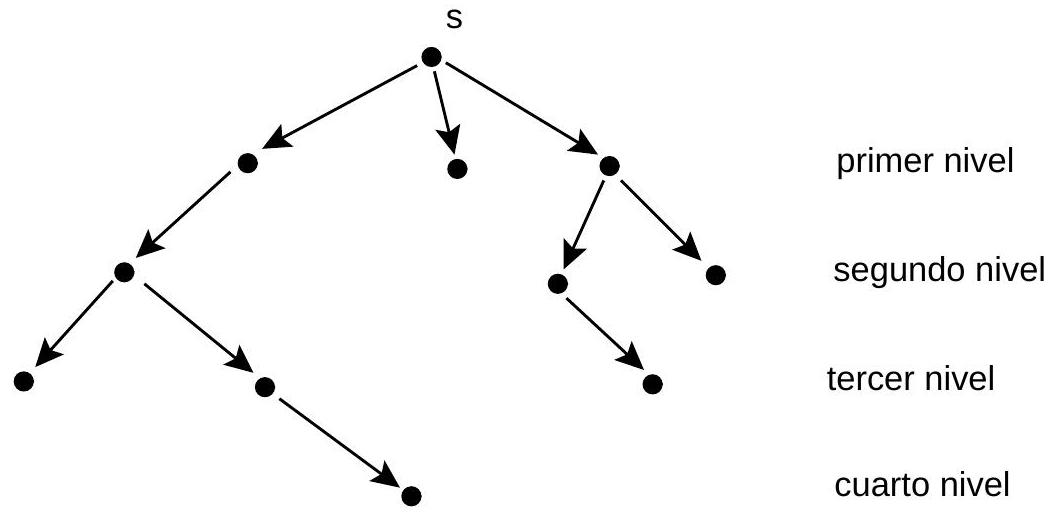
\includegraphics[max width=\textwidth, center]{2025_09_05_458e5b1ce89abceb5d44g-15}\\
es un árbol dirigido con raíz $s$ y cuatro niveles.\\
Observación 3.5. Si un árbol dirigido con raíz es binario y tiene $n$ niveles entonces tiene $2^{n+1}-1$ vértices.\\
Consideremos el siguiente problema: dado un árbol dirigido con raíz $s$, donde cada vértice $x$ tiene asignado un costo $c(x)$ que satisface $c(x) \leq c(y)$ para toda rama ( $x, y$ ) queremos hallar una hoja de mínimo costo.

Describiremos un algoritmo, conocido como branch and bound, que resuelve este problema. El procedimiento utiliza una mezcla de backtracking (volver al vértice anterior para examinar alguno de sus hijos que todavía no ha sido examinado) y un criterio particular de poda que consiste en eliminar toda la descendencia de un vértice $x$ cuando se satisfaga que $c(x) \geq c(h)$ para alguna hoja $h$ encontrada previamente (es decir, cuando ninguna hoja descendiente de $x$ puede ser la solución óptima del problema).

\section*{Descripción del algoritmo.}
\begin{enumerate}
  \setcounter{enumi}{-1}
  \item $L=\{s\}, c=\infty$.
  \item Si $x$ es, de los elementos de $L$, el último que ingresó, $L=L-\{x\}$. Calcular $c(x)$. Si $c(x) \geq c$, goto 4 .
  \item Si $x$ no es una hoja, $L=L \cup\{$ hijos de $x\}$, goto 4 .
  \item $h=x, c=c(x)$.
  \item Si $L \neq \emptyset$ goto 1 .
  \item STOP.
\end{enumerate}

Ejemplo 3.6. Consideremos el árbol dirigido con raíz $s$\\
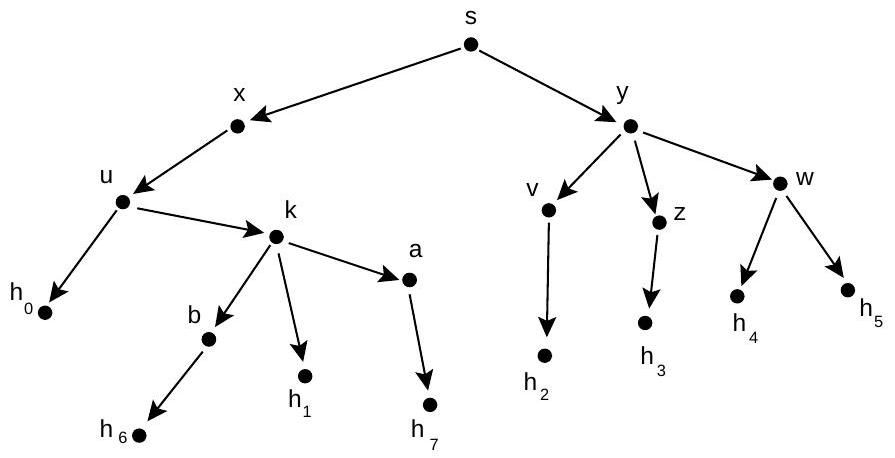
\includegraphics[max width=\textwidth, center]{2025_09_05_458e5b1ce89abceb5d44g-16}\\
donde $c(s)=3, c(x)=4, c(y)=4, c(z)=4, c(u)=7, c(v)=8, c(w)=7, c(k)=10, c(a)=12, c(b)=13$, $c\left(h_{0}\right)=8, c\left(h_{1}\right)=11, c\left(h_{2}\right)=9, c\left(h_{3}\right)=6, c\left(h_{4}\right)=8$ y $c\left(h_{5}\right)=11, c\left(h_{6}\right)=14, c\left(h_{7}\right)=14$.

Aplicando el algoritmo obtenemos\\
0. $L=\{s\}, c=\infty$.

\begin{enumerate}
  \item $L=\emptyset, c(s)=3$.
  \item $L=\{x, y\}$, goto 4 .
  \item $L \neq \emptyset$, goto 1 .
  \item $L=\{x\}, c(y)=4<\infty=c$.
  \item $L=\{x, v, z, w\}$, goto 4 .
  \item $L \neq \emptyset$, goto 1 .
  \item $L=\{x, v, z\}, c(w)=7<\infty=c$.
  \item $L=\left\{x, v, z, h_{4}, h_{5}\right\}$, goto 4 .
  \item $L \neq \emptyset$, goto 1 .
  \item $L=\left\{x, v, z, h_{4}\right\}, c\left(h_{5}\right)=11<\infty=c$.
  \item $h=h_{5}, c=11$.
  \item $L \neq \emptyset$, goto 1 .
  \item $L=\{x, v, z\}, c\left(h_{4}\right)=8<11=c$.
  \item $h=h_{4}, c=8$.
  \item $L \neq \emptyset$, goto 1 .
  \item $L=\{x, v\}, c(z)=4<8=c$.
  \item $L=\left\{x, v, h_{3}\right\}$, goto 4 .
  \item $L \neq \emptyset$, goto 1 .
  \item $L=\{x, v\}, c\left(h_{3}\right)=6<8=c$.
  \item $h=h_{3}, c=6$.
  \item $L \neq \emptyset$, goto 1 .
  \item $L=\{x\}, c(v)=8 \geq 6=c$, goto 4 .
  \item $L \neq \emptyset$, goto 1 .
  \item $L=\emptyset, c(x)=4<6=c$.
  \item $L=\{u\}$, goto 4 .
  \item $L \neq \emptyset$, goto 1 .
  \item $L=\emptyset, c(u)=7 \geq 6=c$, goto 4 .
  \item $L \neq \emptyset$.
  \item STOP.
\end{enumerate}

El siguiente gráfico es una interpretación de los pasos seguidos por el algoritmo en nuestro ejemplo.\\
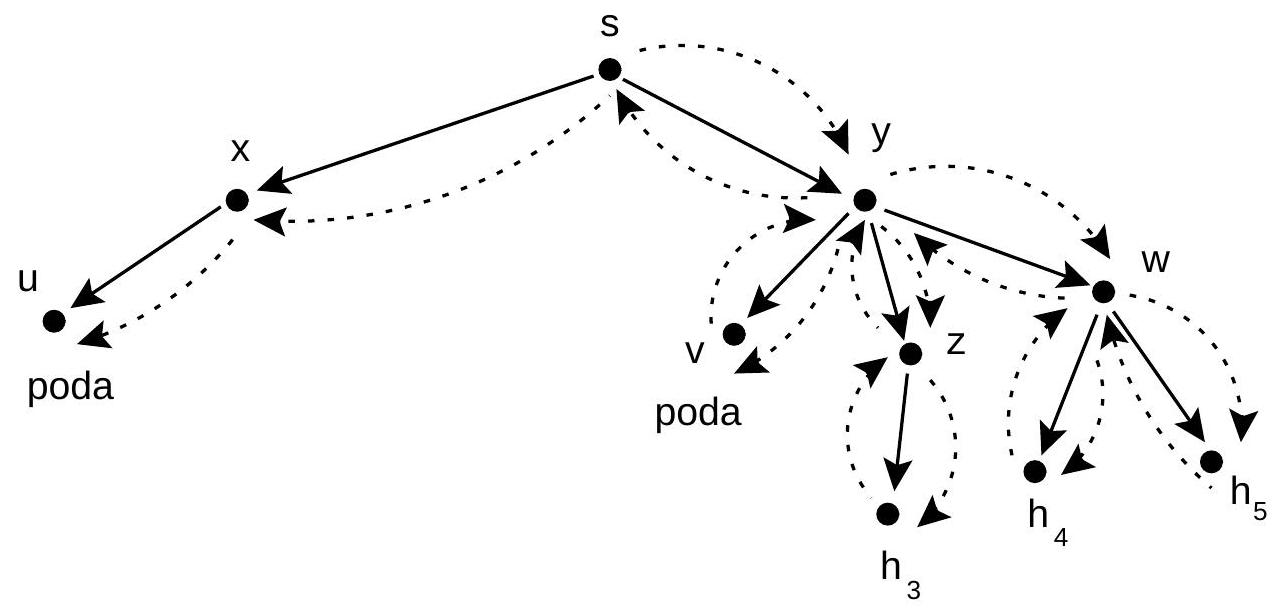
\includegraphics[max width=\textwidth, center]{2025_09_05_458e5b1ce89abceb5d44g-17}

Los vértices son examinados en el orden en que indican las flechas punteadas descendentes. Cada flecha punteada ascendente indica un backtracking. El valor de $c$ en cada iteración del algoritmo es el costo de la hoja más barata encontrada hasta el momento y $h$ guarda la información de cuál es la hoja cuyo costo es $c$ (cuando el algoritmo encuentra una hoja de costo menor que el valor de $c$ presente en ese momento, actualiza $c$ y $h$ ).\\
Si al examinar un nodo $i$ resulta que $c(i) \geq c$ entonces toda su descendencia es podada ya que ninguna hoja que sea un descendiente de $i$ puede tener costo menor que $c$, es decir, costo menor que el de la hoja más barata hallada hasta ese momento.

Como una hoja no es examinada por el algoritmo sólo cuando es seguro que no puede ser una solución óptima entonces en alguna iteración del algoritmo una hoja de mínimo costo es examinada. Cuando el algoritmo encuentra la primer hoja de mínimo costo los valores de $h$ y $c$ son actualizados ya que su costo es menor que el valor de $c$ que estaba presente en ese momento, y a partir de allí $c$ y $h$ permanecen constantes hasta terminar el algoritmo ya que ninguna otra hoja encontrada más tarde puede tener costo menor que el de esta hoja de mínimo costo. Luego, al terminar el algoritmo la hoja que se encuentra almacenada en $h$ es una hoja de mínimo costo y $c=c(h)$.\\
Luego, en este caso, la hoja de mínimo costo es $h=h_{3}$, con costo $c=6$.\\
En este ejemplo la función $c(x)$ estaba dada explícitamente. Esto no es así en general, sino que es una función que se deberá calcular.

En el caso en que la función $c$ satisfaga $c(x) \geq c(y)$ para toda rama $(x, y)$, podemos resolver el problema de hallar una hoja de máximo costo utilizando el algoritmo que resulta de reemplazar, en el paso $0 ., c=\infty$ por $c=-\infty$ y, en el paso 1., la condición $c(x) \geq c$ por la condición $c(x) \leq c$, es decir, el algoritmo\\
$0^{\prime} . L=\{s\}, c=-\infty$.\\
$1^{\prime}$. Sea $x$ es el último vértice que ingresó en $L, L=L-\{x\}$. Calcular $c(x)$. Si $c(x) \leq c$, goto 4 .\\
2'. Si $x$ no es una hoja, $L=L \cup\{$ hijos de $x\}$, goto 4 .\\
3'. $h=x, c=c(x)$.\\
4'. Si $L \neq \emptyset$ goto 1 .\\
5'. STOP.

\section*{4. Aplicación al problema de programación lineal entera.}
Consideremos el problema de programación lineal


\begin{align*}
& \min c x \\
& A x \leq b  \tag{12}\\
& 0 \leq x_{j} \leq u_{j} \quad(1 \leq j \leq n)
\end{align*}


donde $u_{j}<\infty$ para todo $j$ y consideremos el problema de programación lineal entera que resulta de agregar a (12) la restricción adicional


\begin{equation*}
x_{i} \text { entero } \quad(1 \leq i \leq m) \tag{13}
\end{equation*}


donde $m \leq n$ es un número natural dado. Resolveremos este problema de programación lineal entera generando un árbol binario dirigido cuya raíz será el problema (12) y los restantes vértices serán subproblemas que resulten de agregar a (12) ciertas resticciones del tipo $x_{j} \leq k$ o $x_{j} \geq k+1$ para algunos $j$. Las hojas serán los subproblemas cuyas solución óptima verifica la restricción (13) y los subproblemas que no sean factibles. Para cada vértice $u$ definiremos $c(u)$ como el valor del funcional en la solución óptima del subproblema $u$ si este es factible y definiremos $c(u)=\infty$ si el subproblema $u$ no es factible. La función $c(u)$ verificará $c(u) \leq c(v)$ para toda rama $(u, v)$ del árbol. Usaremos el método de branch and bound para encontrar una hoja de mínimo costo y eso nos dará la solución del problema de programación lineal entera.

Observación 4.1. La condición $0 \leq x_{j} \leq u_{j}$ asegura que el poliedro definido por las restricciones es acotado. Como también es cerrado (pues es intersección finita de de semiespacios del tipo $\{x / a . x \leq b\}$ o $\{x / a . x \geq b\}$ que son cerrados) entonces es compacto. Luego, si (12) es factible entonces siempre existe una solución óptima ya que el funcional es una función contínua y toda función contínua sobre un compacto alcanza su máximo y su mínimo. Lo mismo vale para cualquier subproblema que resulte de agregar a (12) restricciones del tipo $x_{j} \leq k$ o $x_{j} \geq k+1$ para algunos $j$.

Observación 4.2. Si $z^{*}$ es el valor del funcional en una solución óptima de un problema $u$ de programación lineal y $z$ es el valor del funcional en el óptimo de cualquier subproblema $v$ que se obtenga agregándole una restricción a $u$ entonces $z^{*} \leq z$ ya que toda solución óptima del subproblema $v$ es una solución factible del problema $u$. Notemos también que si el problema fuese maximizar el funcional en lugar de minimizarlo entonces tendríamos que $z^{*} \geq z$.\\
Veamos ahora con más detalle cómo construír el árbol.\\
La raíz $s$ del árbol es el problema (12). Notemos que toda solución factible del problema de programación lineal entera es una solución factible de $s$. Supongamos que hemos construído una parte del árbol donde cada vértice es un subproblema que resulta de agregar a (12) restricciones del tipo $x_{j} \leq k$ o $x_{j} \geq k+1$ para algunos $j$, donde $k$ es un entero no negativo y tal que toda solución factible del problema de programación\\
lineal entera es una solución factible de alguna hoja de este subárbol. Para cada subproblema $u$ que sea una hoja del subárbol que tenemos construído hasta ahora (es decir, cada vértice $u$ que no tenga hijos) hacemos lo siguiente:\\
Si $u$ tiene una solución óptima que no satisface (13), sea $j(1 \leq j \leq m)$ el primer índice para el cual $x_{j}$ no es entero y sea $r$ un entero tal que $r<x_{j}<r+1$. Entonces creamos dos hijos de $u$, uno agregando al problema $u$ la restricción $x_{j} \leq r$ y el otro agregando a $u$ la restricción $x_{j} \geq r+1$. Notemos que si una solución factible del problema de programación lineal entera es una solución factible de $u$ entonces es una solución factible de alguno de los hijos de $u$ ya que, como $r$ es entero, si la $j$-ésima coordenada de esta solución es entera entonces o bien es menor o igual que $r$ o bien es mayor o igual que $r+1$.\\
Si en cambio $u$ tiene una solución óptima que satisface (13) o si no tiene soluciones factibles (notar que, por la observación 4.1., si $u$ es factible entonces necesariamente tiene una solución óptima) entonces no creamos ningún hijo de $u$.\\
De esta manera obtenemos un árbol binario dirigido con raíz $s$ cuyas hojas son los subproblemas cuyas solución óptima verifica la restricción (13) y los subproblemas que no sean factibles. Además, toda solución factible del problema de programación lineal entera es una solución factible de alguna hoja del árbol.\\
Para cada vértice $u$ de este árbol definimos $c(u)$ como el valor del funcional en la solución óptima del subproblema $u$ si este es factible y $c(u)=\infty$ si no. Debido a la forma en que hemos construído el árbol esta función satisface $c(u) \leq c(v)$ para toda rama $(u, v)$ del árbol ya que si $(u, v)$ es una rama del árbol entonces $v$ es un subproblema que se obtuvo agreagando una restricción a $u$ (ver observación 4.2.). De esta manera, el costo de una hoja que corresponda a un problema factible será el valor del funcional en una solución factible del problema de programación lineal entera. Como las soluciones factibles del problema de programación lineal entera son las soluciones factibles de cada una de las hojas del árbol entonces una hoja de mínimo costo será una solución óptima del problema de programación lineal entera.\\
Para hallar una hoja de mínimo costo utilizaremos el método de branch and bound, pero en lugar de generar todo el árbol y luego aplicar el algoritmo, en cada paso del algoritmo calcularemos sólo los vértices y los costos que necesitemos. Es decir, cada vez que realizamos el paso 1. debemos resolver el subproblema $x$ para el último vértice $x$ que ingresó en $L$ y en el caso en que no sea una hoja generamos los dos hijos de $x$ que ingresaremos en $L$ en el siguiente paso. De esta manera evitamos calcular las ramas que luego el algoritmo podaría.

En el caso en que el problema sea de maximización entonces la función $c(u)$ se define como el valor del funcional en el subproblema $u$ si $u$ es factible y como $c(u)=-\infty$ si no y satisface $c(u) \geq c(v)$ para toda rama ( $u, v$ ) del árbol (ver observación 4.2.). En este caso lo que buscamos es una hoja de máximo costo.

Ejemplo 4.3. Resolveremos el problema de programación lineal entera

$$
\begin{aligned}
& \max 3 x_{1}+3 x_{2}+13 x_{3} \\
& -3 x_{1}+6 x_{2}+7 x_{3} \leq 8 \\
& 6 x_{1}-3 x_{2}+7 x_{3} \leq 8 \\
& 0 \leq x_{i} \leq 5 \quad x_{i} \text { entero }
\end{aligned}
$$

$0^{\prime} . L=\{s\}, c=-\infty$\\
donde la raíz del árbol es el problema


\begin{align*}
& \max 3 x_{1}+3 x_{2}+13 x_{3} \\
& -3 x_{1}+6 x_{2}+7 x_{3} \leq 8 \\
& 6 x_{1}-3 x_{2}+7 x_{3} \leq 8  \tag{s}\\
& \quad 0 \leq x_{i} \leq 5
\end{align*}


1'. $L=\emptyset$. Calculamos $c(s)$. Para ello resolvemos el problema $s$. En este caso una solución óptima es $\left(x_{1}, x_{2}, x_{3}\right)=\left(\frac{8}{3}, \frac{8}{3}, 0\right)$ y el valor del funcional en ella es 16. Luego $c(s)=16$. Como $c(s)$ es mayor que $c=-\infty$ vamos a $2^{\prime}$.\\
2'. $s$ no es una hoja, ya que $x_{1}$ no es entero. Como $2<x_{1}<3$, los hijos de $s$ son los subproblemas $u_{1}$ y $u_{2}$ que resultan de agregar al problema $s$ las restricciones $x_{1} \leq 2$ y $x_{1} \geq 3$ respectivamente. Es decir,

$$
\begin{array}{ccc}
\max 3 x_{1}+3 x_{2}+13 x_{3} & & \max 3 x_{1}+3 x_{2}+13 x_{3} \\
-3 x_{1}+6 x_{2}+7 x_{3} \leq 8 & & -3 x_{1}+6 x_{2}+7 x_{3} \leq 8 \\
6 x_{1}-3 x_{2}+7 x_{3} \leq 8 & \left(u_{1}\right) & \mathrm{y} \\
x_{1} \leq 2 & & 6 x_{1}-3 x_{2}+7 x_{3} \leq 8 \\
0 \leq x_{i} \leq 5 & & x_{1} \geq 3 \\
\left(u_{2}\right) \\
\end{array}
$$

Actualizamos $L$ en la forma $L=\left\{u_{1}, u_{2}\right\}$\\
$4^{\prime}$. $L \neq \emptyset$, vamos a $1^{\prime}$.\\
$1^{\prime}$. $L=\left\{u_{1}\right\}$. Calculamos $c\left(u_{2}\right)$. En este caso $u_{2}$ no es factible. Luego, $c\left(u_{2}\right)=-\infty$. Como $c\left(u_{2}\right)$ es menor o igual que $c=-\infty$ vamos a $4^{\prime}$.\\
$4^{\prime}$. $L \neq \emptyset$, vamos a $1^{\prime}$.\\
$1^{\prime}$. $L=\emptyset$. Calculamos $c\left(u_{1}\right)$. Para ello resolvemos $u_{1}$. Una solución óptima es $\left(x_{1}, x_{2}, x_{3}\right)=\left(2,2, \frac{2}{7}\right)$ y el valor del funcional en ella es $15+\frac{5}{7}$, de donde $c\left(u_{1}\right)=15+\frac{5}{7}$. Como $c\left(u_{1}\right)$ es mayor que $c=-\infty$ vamos a 2 '. 2 '. $u_{1}$ no es una hoja, ya que $x_{3}$ no es entero. Como $0<x_{3}<1$, los hijos de $u_{1}$ son los subproblemas $u_{3}$ y $u_{4}$ que resultan de agregar al problema $u_{1}$ las restricciones $x_{3} \leq 0$ y $x_{3} \geq 1$ respectivamente. Es decir,

\[
\begin{array}{ccc}
\max 3 x_{1}+3 x_{2}+13 x_{3} & & \max 3 x_{1}+3 x_{2}+13 x_{3} \\
-3 x_{1}+6 x_{2}+7 x_{3} \leq 8 & & \\
6 x_{1}-3 x_{2}+7 x_{3} \leq 8 & \left(u_{3}\right) & \mathrm{y} \\
x_{1} \leq 2 & & 6 x_{1}-3 x_{2}+7 x_{3} \leq 8  \tag{4}\\
x_{3} \leq 0 & & x_{1} \leq 2 \\
0 \leq x_{i} \leq 5 & & x_{3} \geq 1 \\
& & 0 \leq x_{i} \leq 5
\end{array}
\]

Actualizamos $L$ en la forma $L=\left\{u_{3}, u_{4}\right\}$\\
$4^{\prime}$. $L \neq \emptyset$, vamos a $1^{\prime}$.\\
$1^{\prime}$. $L=\left\{u_{3}\right\}$. Calculamos $c\left(u_{4}\right)$. Una solución óptima de $u_{4}$ es $\left(x_{1}, x_{2}, x_{3}\right)=\left(\frac{1}{3}, \frac{1}{3}, 1\right)$ y el valor del funcional en ella es $c\left(u_{4}\right)=15$. Como $c\left(u_{4}\right)$ es mayor que $c=-\infty$ vamos a 2 '.\\
2 '. $u_{4}$ no es una hoja ya que $x_{1}$ no es entero. Como $0<x_{1}<1$ los hijos de $u_{4}$ son los subproblemas $u_{5}$ y $u_{6}$ que resultan de agregar al problema $u_{4}$ las restricciones $x_{1} \leq 0$ y $x_{1} \geq 1$ respectivamente. Es decir,

$$
\begin{array}{ccc}
\max 3 x_{1}+3 x_{2}+13 x_{3} & & \max 3 x_{1}+3 x_{2}+13 x_{3} \\
-3 x_{1}+6 x_{2}+7 x_{3} \leq 8 & & -3 x_{1}+6 x_{2}+7 x_{3} \leq 8 \\
6 x_{1}-3 x_{2}+7 x_{3} \leq 8 & & 6 x_{1}-3 x_{2}+7 x_{3} \leq 8 \\
x_{1} \leq 2 & \left(u_{5}\right) & \mathrm{y} \\
x_{3} \geq 1 & & x_{1} \leq 2 \\
x_{1} \leq 0 & & x_{3} \geq 1 \\
0 \leq x_{i} \leq 5 & & x_{1} \geq 1 \\
& & 0 \leq x_{i} \leq 5
\end{array}
$$

Actualizamos $L$ en la forma $L=\left\{u_{3}, u_{5}, u_{6}\right\}$\\
$4^{\prime} . L \neq \emptyset$, vamos a $1^{\prime}$.\\
$1^{\prime}$. $L=\left\{u_{3}, u_{5}\right\}$. Calculamos $c\left(u_{6}\right)$. El problema $u_{6}$ no es factible. Luego, $c\left(u_{6}\right)=-\infty$. Como $c\left(u_{6}\right)$ es menor o igual que $c=-\infty$ vamos a $4^{\prime}$.\\
$4^{\prime} . L \neq \emptyset$, vamos a $1^{\prime}$.\\
$1^{\prime}$. $L=\left\{u_{3}\right\}$. Calculamos $c\left(u_{5}\right)$. Una solución óptima de $u_{5}$ es $\left(x_{1}, x_{2}, x_{3}\right)=\left(0,0, \frac{8}{7}\right)$ y el valor del funcional en ella es $c\left(u_{5}\right)=14+\frac{6}{7}$. Como $c\left(u_{5}\right)$ es mayor que $c=-\infty$ vamos a $2^{\prime}$.\\
$2^{\prime}$. $u_{5}$ no es una hoja ya que $x_{3}$ no es entero. Como $1<x_{1}<2$ los hijos de $u_{5}$ son los subproblemas $u_{7}$ y $u_{8}$ que resultan de agregar al problema $u_{5}$ las restricciones $x_{3} \leq 1$ y $x_{3} \geq 2$ respectivamente. Es decir,

\[
\begin{array}{ccc}
\max 3 x_{1}+3 x_{2}+13 x_{3} & & \max 3 x_{1}+3 x_{2}+13 x_{3} \\
-3 x_{1}+6 x_{2}+7 x_{3} \leq 8 & & -3 x_{1}+6 x_{2}+7 x_{3} \leq 8 \\
6 x_{1}-3 x_{2}+7 x_{3} \leq 8 & & 6 x_{1}-3 x_{2}+7 x_{3} \leq 8 \\
x_{1} \leq 2 & \left(u_{7}\right) & \mathrm{y} \\
x_{3} \geq 1 & & x_{1} \leq 2  \tag{8}\\
x_{1} \leq 0 & & x_{3} \geq 1 \\
x_{3} \leq 1 & & x_{1} \leq 0 \\
0 \leq x_{i} \leq 5 & & x_{3} \geq 2 \\
& & 0 \leq x_{i} \leq 5
\end{array}
\]

Actualizamos $L$ en la forma $L=\left\{u_{3}, u_{7}, u_{8}\right\}$\\
$4^{\prime} . L \neq \emptyset$, vamos a $1^{\prime}$.\\
$1^{\prime}$. $L=\left\{u_{3}, u_{7}\right\}$. Calculamos $c\left(u_{8}\right)$. El problema $u_{8}$ no es factible. Luego, $c\left(u_{8}\right)=-\infty$. Como $c\left(u_{8}\right)$ es menor o igual que $c=-\infty$ vamos a $4^{\prime}$.\\
$4^{\prime} . L \neq \emptyset$, vamos a $1^{\prime}$.\\
$1^{\prime}$. $L=\left\{u_{3}\right\}$. Calculamos $c\left(u_{7}\right)$. Una solución óptima de $u_{7}$ es $\left(x_{1}, x_{2}, x_{3}\right)=(0,0,1)$ y el valor del funcional en ella es $c\left(u_{7}\right)=13$. Como $c\left(u_{7}\right)$ es mayor que $c=-\infty$ vamos a $2^{\prime}$.

2'. Como $u_{7}$ es una hoja, no modificamos $L$ y vamos a $3^{\prime}$.\\
3'. $h=u_{7}, c=c\left(u_{7}\right)=13$\\
$4^{\prime}$. $L \neq \emptyset$, vamos a $1^{\prime}$.\\
$1^{\prime}$. $L=\emptyset$. Calculamos $c\left(u_{3}\right)$. Una solución óptima de $u_{3}$ es $\left(x_{1}, x_{2}, x_{3}\right)=\left(2, \frac{7}{3}, 0\right)$ y el valor del funcional en ella es $c\left(u_{3}\right)=13$. Como $c\left(u_{3}\right)$ es menor o igual que $c=13$ vamos a $4^{\prime}$.

4'. Como $L=\emptyset$, vamos a $5^{\prime}$.\\
5'. STOP.

Luego, la hoja de máximo costo es $h=u_{7}$ con costo $c=13$. Esto significa que una solución óptima del problema de programación lineal entera que queríamos resolver es $\left(x_{1}, x_{2}, x_{3}\right)=(0,0,1)$ y el valor del funcional en ella es $c\left(u_{7}\right)=13$.

El subárbol generado por el algoritmo es\\
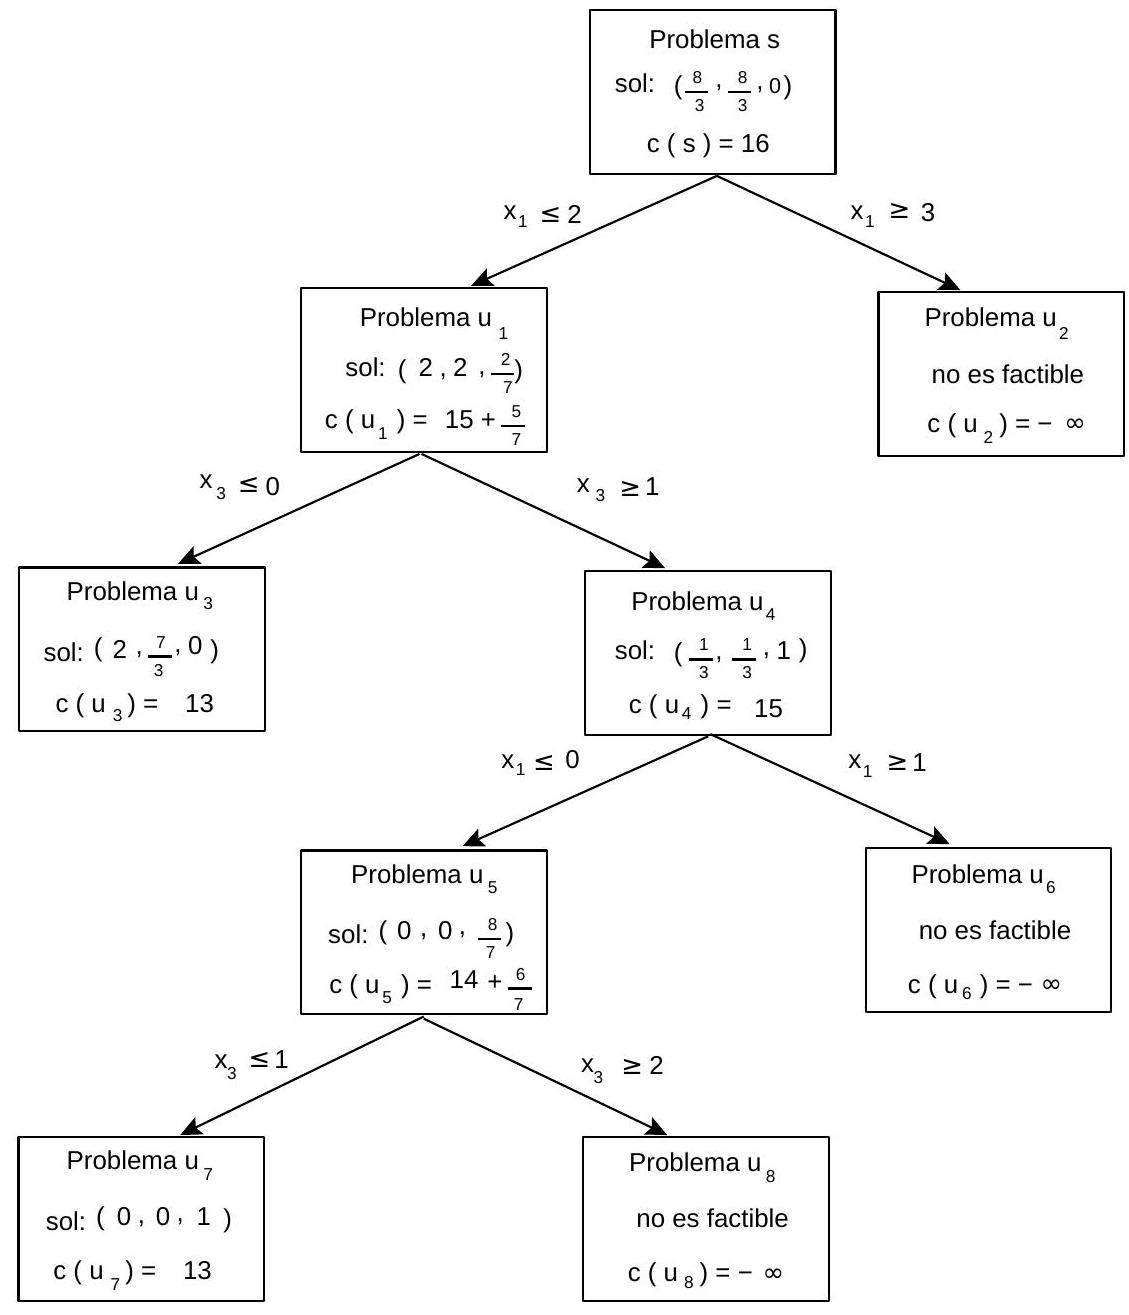
\includegraphics[max width=\textwidth, center]{2025_09_05_458e5b1ce89abceb5d44g-22}

\section*{5. Aplicación de branch and bound al problema del viajante.}
Como vimos, el problema del viajante puede plantearse por programación lineal entera (ver ejemplo 1.9.) y por lo tanto resolverse utilizando el método de branch and bound en la forma descripta en la sección anterior. Veremos ahora otro algoritmo para resolver este problema, esencialmente distinto pero que también utiliza el método de branch and bound.\\
Sea $G=(V, E)$ un grafo completo dirigido, donde $V=\{1, \ldots, n\}$ y donde cada rama $(i, j)$ de $G$ tiene asignado un costo $c_{i j}$ tal que $0 \leq c_{i j} \leq \infty$.\\
Recordemos que un circuito Hamiltoniano $\mathcal{C}$ es un ciclo dirigido en $G$ que pasa por cada vértice una y sólo una vez. El costo $c(\mathcal{C})$ del circuito se define como la suma de los costos de las ramas que lo forman, es decir,

$$
c(\mathcal{C})=\sum_{(i, j) \in \mathcal{C}} c_{i j}
$$

El problema consiste en hallar un circuito Hamiltoniano $\mathcal{C}$ de mínimo costo.\\
Como antes, para resolver este problema generaremos un árbol binario dirigido con raíz y definiremos una función $c(u)$ conveniente que satisfaga $c(u) \leq c(v)$ para toda rama $(u, v)$ de manera que nuestro problema\\
se traduzca en hallar una hoja de mínimo costo. De ahora en más, la palabra circuito significará circuito Hamiltoniano.\\
La raíz del árbol será el problema del viajante, es decir, hallar un circuito $\mathcal{C}$ tal que $c(\mathcal{C})$ sea mínimo. Supongamos que hemos construído una parte del árbol donde cada vértice es un subproblema que resulta de agregar a su vértice padre la restricción $(i, j) \in \mathcal{C}$ o la restricción $(i, j) \notin \mathcal{C}$, para cierta rama $(i, j) \in E$.\\
Para cada subproblema $u$ que sea una hoja del subárbol que tenemos construído hasta ahora hacemos lo siguiente:\\
Sea $A_{u}=\{e \in E /$ " $e \in \mathcal{C}$ " es una restricción de $u\}$.\\
Si $\# A_{u}<n-1$ entonces elegimos convenientemente una rama $(i, j) \in E$ y generamos dos hijos de $u$, uno agregando a $u$ la restricción $(i, j) \in \mathcal{C}$ y el otro agregando a $u$ la restricción $(i, j) \notin \mathcal{C}$.\\
Si, en cambio, $\# A_{u}=n-1$ entonces no generamos ningún hijo de $u$.\\
Veamos en un ejemplo cuál es la manera en que se eligen las ramas $(i, j)$ que definen las restricciones de los subproblemas, cómo calcular el costo de cada vértice del árbol que se genera y la razón por la cual el problema se traduce en encontrar una hoja de mínimo costo.

En lo que sigue, por número entenderemos un número real o infinito. Sea $G$ el grafo completo dirigido con los $n=7$ vértices $1,2, \ldots 7$. Supongamos que el costo de cada rama $(i, j)$ de $G(1 \leq i, j \leq 7)$ está dado por la matriz

$$
\left\|c_{i j}\right\|=\left(\begin{array}{ccccccc}
\infty & 3 & 93 & 13 & 33 & 9 & 57 \\
4 & \infty & 77 & 42 & 21 & 16 & 34 \\
45 & 17 & \infty & 36 & 16 & 28 & 25 \\
39 & 90 & 80 & \infty & 56 & 7 & 91 \\
28 & 46 & 88 & 33 & \infty & 25 & 57 \\
3 & 88 & 18 & 46 & 92 & \infty & 7 \\
44 & 26 & 33 & 27 & 84 & 39 & \infty
\end{array}\right)
$$

Paso 1. Definimos la raíz $s$ del árbol como el problema de hallar un circuito $\mathcal{C}$ tal que $c(\mathcal{C})$ sea mínimo.\\
Paso 2. Calculamos el costo y generamos los hijos de cada nodo $u$ que sea una hoja del subárbol que tenemos construído hasta ahora y que satisfaga que $\# A_{u}<n-1$.\\
El subárbol que tenemos construído hasta ahora tiene un solo nodo (la raíz $s$ ), que es una hoja. Como $\# A_{s}=0<6=n-1$ pues $A_{s}=\emptyset$, para calcular $c(s)$ y generar los hijos de $s$ procedemos de la siguiente manera:

Asociamos a $s$ la matriz $\left\|c_{i j}(s)\right\|=\left\|c_{i j}\right\|$ y consideremos la matriz $D_{1}$ que se obtiene restando un número no negativo $k_{1}$ a cada coeficiente de la fila 1 de $\left\|c_{i j}(s)\right\|$ de manera que cada coeficiente de la nueva matriz sea no negativo. Como cada circuito $\mathcal{C}$ pasa una sola vez por el vértice 1 entonces existe un único $j, 1 \leq j \leq 7, j \neq 1$ tal que la rama $(1, j) \in \mathcal{C}$. Luego el costo de cualquier circuito $\mathcal{C}$ calculado utilizando la nueva matriz de costos $D_{1}$ es igual a $c(\mathcal{C})-k_{1}$ ya que la única rama cuyo costo sufrió una modificación es la rama $(1, j)$ cuyo costo fue disminuido en $k_{1}$.\\
Hacemos esto con el máximo valor posible de $k_{1}$, en este caso $k_{1}=3$, para que la nueva matriz $D_{1}$ tenga al menos un coeficiente nulo en la primera fila. Ahora consideremos la matriz $D_{2}$ que se obtiene restando un número no negativo $k_{2}$ a cada coeficiente de la fila 2 de $D_{1}$ de manera que cada coeficiente de la nueva matriz sea no negativo. Como cada circuito $\mathcal{C}$ pasa una sola vez por el vértice 2 entonces existe un único $j$, $1 \leq j \leq 7, j \neq 2$ tal que la rama $(2, j) \in \mathcal{C}$. Luego el costo de cualquier circuito $\mathcal{C}$ calculado utilizando la nueva matriz de costos $D_{2}$ es igual al costo de $\mathcal{C}$ calculado usando la matriz de costos $D_{1}$ menos $k_{2}$, lo que es igual a $c(\mathcal{C})-k_{1}-k_{2}$.\\
Hacemos esto con el máximo valor posible de $k_{2}$, en este caso $k_{2}=4$. De esta manera $D_{2}$ tiene al menos un coeficiente nulo en cada una de las dos primeras filas.

Repitiendo este procedimiento para las restantes filas obtenemos la matriz

$$
D_{n}=D_{7}=\left(\begin{array}{ccccccc}
\infty & 0 & 90 & 10 & 30 & 6 & 54 \\
0 & \infty & 73 & 38 & 17 & 12 & 30 \\
29 & 1 & \infty & 20 & 0 & 12 & 9 \\
32 & 83 & 73 & \infty & 49 & 0 & 84 \\
3 & 21 & 63 & 8 & \infty & 0 & 32 \\
0 & 85 & 15 & 43 & 89 & \infty & 4 \\
18 & 0 & 7 & 1 & 58 & 13 & \infty
\end{array}\right)
$$

que tiene al menos un coeficiente nulo en cada fila. El costo de cualquier circuito $\mathcal{C}$ calculado utilizando la nueva matriz de costos $D_{n}$ es $c(\mathcal{C})-k_{1}-k_{2}-\cdots-k_{7}$, donde $k_{1}=3, k_{2}=4, k_{3}=16, k_{4}=7, k_{5}=25$, $k_{6}=3$ y $k_{7}=26$. Ahora, para cada $j,(1 \leq j \leq 7)$ restamos un número no negativo $r_{j}$ a cada coeficiente de la columna $j$ de $D_{n}$ de manera que cada coeficiente de la nueva matriz sea no negativo. Eligiendo $r_{j}$ el máximo valor posible, en este caso $r_{1}=0, r_{2}=0, r_{3}=7, r_{4}=1, r_{5}=0, r_{6}=0$ y $r_{7}=4$, obtenemos la matriz

$$
\left\|c_{i j}^{\prime}(s)\right\|=\left(\begin{array}{ccccccc}
\infty & 0 & 83 & 9 & 30 & 6 & 50 \\
0 & \infty & 66 & 37 & 17 & 12 & 26 \\
29 & 1 & \infty & 19 & 0 & 12 & 5 \\
32 & 83 & 66 & \infty & 49 & 0 & 80 \\
3 & 21 & 56 & 7 & \infty & 0 & 28 \\
0 & 85 & 8 & 42 & 89 & \infty & 0 \\
18 & 0 & 0 & 0 & 58 & 13 & \infty
\end{array}\right)
$$

que tiene al menos un coeficiente nulo en cada fila y en cada columna. El costo de cualquier circuito $\mathcal{C}$ calculado utilizando la nueva matriz de costos $\left\|c_{i j}^{\prime}(s)\right\|$ definido por

$$
c^{\prime}(\mathcal{C}, s)=\sum_{(i, j) \in \mathcal{C}} c_{i j}^{\prime}(s)
$$

satisface $c^{\prime}(\mathcal{C}, s)=c(\mathcal{C})-k_{1}-\cdots-k_{7}-r_{1}-\cdots-r_{7}$. Definimos $c(s)=k_{1}+\cdots+k_{n}+r_{1}+\cdots+r_{n}$. En este caso, $c(s)=96$. De esta manera, $c(\mathcal{C})=c^{\prime}(\mathcal{C}, s)+c(s)=c^{\prime}(\mathcal{C}, s)+96$.

Observación 5.1. Para cualquier circuito $\mathcal{C}$ se verifica que $c(\mathcal{C}) \geq c(s)$. En efecto, como los coeficientes de $\left\|c_{i j}^{\prime}(s)\right\|$ son no negativos entonces $c^{\prime}(\mathcal{C}, s) \geq 0$. Luego, $c(\mathcal{C})=c^{\prime}(\mathcal{C}, s)+c(s) \geq c(s)$.

Ahora generamos dos hijos $u_{1}$ y $v_{1}$ de $s$, eligiendo una rama $\left(i_{1}, j_{1}\right) \in E$ tal que el coeficiente $c_{i_{1} j_{1}}^{\prime}(s)$ correspondiente a la fila $i_{1}$ y a la columna $j_{1}$ de $\left\|c_{i j}^{\prime}(s)\right\|$ sea nulo, y tomando como $u_{1}$ el subproblema que resulta de agregar al problema $s$ la condición de que ( $i_{1}, j_{1}$ ) pertenezca al circuito y como $v_{1}$ el que resulta de agregar a $s$ la condición de que $\left(i_{1}, j_{1}\right)$ no pertenezca al circuito. Supongamos que en este caso elegimos $\left(i_{1}, j_{1}\right)=(4,6)$. Entonces el subproblema $u_{1}$ es el de hallar un circuito de mínimo costo que contenga a la rama $(4,6)$ y $v_{1}$ el de hallar un circuito de mínimo costo que no la contenga.

Paso 3. Calculamos el costo y generamos los hijos de cada nodo $u$ que sea una hoja del subárbol que tenemos construído hasta ahora y que satisfaga que $\# A_{u}<n-1$.\\
El subárbol que tenemos construído hasta ahora consiste de la raíz $s$ y sus dos hijos, $u_{1}$ y $v_{1}$. Las hojas son, por lo tanto, $u_{1}$ y $v_{1}$.\\
Como $\# A_{u_{1}}=1<6=n-1$ pues $A_{u_{1}}=\left\{\left(i_{1}, j_{1}\right)\right\}$, para calcular $c\left(u_{1}\right)$ y luego generar sus hijos le asociamos al problema $u_{1}$ la matriz de costos $\left\|c_{i j}\left(u_{1}\right)\right\|$ que se obtiene reemplazando en $\left\|c_{i j}^{\prime}(s)\right\|$ el coeficiente $c_{j_{1} i_{1}}^{\prime}(s)$ por $\infty$ y eliminando la fila $i_{1}$ y la columna $j_{1}$.\\
Si $\mathcal{C}$ es un circuito que contiene a la rama ( $i_{1}, j_{1}$ ) entonces para todo $j \neq j_{1}$ la rama ( $i_{1}, j$ ) no puede pertenecer a $\mathcal{C}$, para todo $i \neq i_{1}$ la rama $\left(i, j_{1}\right)$ no puede pertenecer a $\mathcal{C}$. Como además $c_{i_{1} j_{1}}^{\prime}=0$ eso significa que no necesitamos guardar la información sobre la fila $i_{1}$ y la columna $j_{1}$ de $\left\|c_{i j}^{\prime}(s)\right\|$ y por eso\\
son eliminadas. Como además la rama ( $j_{1}, i_{1}$ ) no puede pertenecer al circuito, para evitar que esto pudiera ocurrir reemplazamos el coeficiente $c_{j_{1} i_{1}}^{\prime}(s)$ por $\infty$.\\
Como eliminaremos una fila y una columna, utilizaremos una tabla de doble entrada en lugar de la notación matricial con el objeto de no perder la información de a cuáles ramas corresponden los distintos costos (el costo de cada rama ( $i, j$ ) según $\left\|c_{i j}\left(u_{1}\right)\right\|$ es el valor correspondiente a la fila $i$ y la columna $j$ ).

En nuestro ejemplo la matriz $\left\|c_{i j}\left(u_{1}\right)\right\|$ correspondiente a $u_{1}$ es

\begin{center}
\begin{tabular}{|c|c|c|c|c|c|c|}
\hline
 & $\operatorname{col} 1$ & $\operatorname{col} 2$ & $\operatorname{col} 3$ & $\operatorname{col} 4$ & $\operatorname{col} 5$ & $\operatorname{col} 7$ \\
\hline
fila 1 & $\infty$ & 0 & 83 & 9 & 30 & 50 \\
\hline
fila 2 & 0 & $\infty$ & 66 & 37 & 17 & 26 \\
\hline
fila 3 & 29 & 1 & $\infty$ & 19 & 0 & 5 \\
\hline
fila 5 & 3 & 21 & 56 & 7 & $\infty$ & 28 \\
\hline
fila 6 & 0 & 85 & 8 & $\infty$ & 89 & 0 \\
\hline
fila 7 & 18 & 0 & 0 & 0 & 58 & $\infty$ \\
\hline
\end{tabular}
\end{center}

En este caso, el costo de la rama ( 5,7 ) según esta matriz es 28 , es decir, $c_{57}\left(u_{1}\right)=28$.\\
Ahora generamos la matriz $\left\|c_{i j}^{\prime}\left(u_{1}\right)\right\|$ que se obtiene restando a cada coeficiente de la fila $i$ de $\left\|c_{i j}\left(u_{1}\right)\right\|$ el máximo número no negativo $k_{i}$ y luego restando a cada coeficiente de la columna $j$ el máximo número no negativo $r_{j}$, de manera que cada coeficiente de la nueva matriz resulte ser no negativo y definimos $c\left(u_{1}\right)=c(s)+\sum k_{i}+\sum r_{j}$. Luego $c\left(u_{1}\right) \geq c(s)$. Notemos que $\left\|c_{i j}^{\prime}\left(u_{1}\right)\right\|$ tiene un coeficiente nulo en cada fila y cada columna.\\
En nuestro caso resulta que $k_{5}=3, k_{i}=0$ para $i \neq 5$ y $r_{j}=0$ para todo $j$, de donde $\left\|c_{i j}^{\prime}\left(u_{1}\right)\right\|$ es la matriz

\begin{center}
\begin{tabular}{|c|c|c|c|c|c|c|}
\hline
 & col 1 & col 2 & col 3 & col 4 & col 5 & col 7 \\
\hline
fila 1 & $\infty$ & 0 & 83 & 9 & 30 & 50 \\
\hline
fila 2 & 0 & $\infty$ & 66 & 37 & 17 & 26 \\
\hline
fila 3 & 29 & 1 & $\infty$ & 19 & 0 & 5 \\
\hline
fila 5 & 0 & 18 & 53 & 4 & $\infty$ & 25 \\
\hline
fila 6 & 0 & 85 & 8 & $\infty$ & 89 & 0 \\
\hline
fila 7 & 18 & 0 & 0 & 0 & 58 & $\infty$ \\
\hline
\end{tabular}
\end{center}

y $c\left(u_{1}\right)=c(s)+3=96+3=99$.\\
Si $\mathcal{C}$ es un circuito que contiene a la rama ( $i_{1}, j_{1}$ ) (es decir, una solución factible de $u_{1}$ ) entonces

$$
\begin{aligned}
c(\mathcal{C}) & =c^{\prime}(\mathcal{C}, s)+c(s)= \\
& =\sum_{(i, j) \in \mathcal{C}} c_{i j}^{\prime}(s)+c(s)= \\
& =\sum_{\substack{(i, j) \in \mathcal{C} \\
(i, j) \neq\left(i_{1}, j_{1}\right)}} c_{i j}^{\prime}(s)+c(s)
\end{aligned}
$$

ya que $\left(i_{1}, j_{1}\right)$ fue elegido verificando $c_{i_{1} j_{1}}^{\prime}(s)=0$.\\
Sean

$$
c\left(\mathcal{C}, u_{1}\right)=\sum_{\substack{(i, j) \in \mathcal{C} \\(i, j) \neq\left(i_{1}, j_{1}\right)}} c_{i j}\left(u_{1}\right)
$$

y

$$
c^{\prime}\left(\mathcal{C}, u_{1}\right)=\sum_{\substack{(i, j) \in \mathcal{C} \\(i, j) \neq\left(i_{1}, j_{1}\right)}} c_{i j}^{\prime}\left(u_{1}\right)
$$

Notemos que $c\left(\mathcal{C}, u_{1}\right)$ y $c^{\prime}\left(\mathcal{C}, u_{1}\right)$ están bien definidos pues si $\mathcal{C}$ es un circuito que contiene a la rama $\left(i_{1}, j_{1}\right)$ entonces para todo $(i, j) \in \mathcal{C},(i, j) \neq\left(i_{1}, j_{1}\right)$ vale que $i \neq i_{1}$, que $j \neq j_{1}$ y que $(i, j) \neq\left(j_{1}, i_{1}\right)$.

Como $\left\|c_{i j}\left(u_{1}\right)\right\|$ fue construída eliminando la fila $i_{1}$ y la columna $j_{1}$ de $\left\|c_{i j}^{\prime}(s)\right\|$ y reemplazando $c_{j_{1} i_{1}}^{\prime}(s)$ por $\infty$ entonces para todo $(i, j) \in \mathcal{C},(i, j) \neq\left(i_{1}, j_{1}\right)$ existen los coeficientes $c_{i j}\left(u_{1}\right)$ y $c_{i j}^{\prime}\left(u_{1}\right)$ y vale

$$
\sum_{\substack{(i, j) \in \mathcal{C} \\(i, j) \neq\left(i_{1}, j_{1}\right)}} c_{i j}^{\prime}(s)=\sum_{\substack{(i, j) \in \mathcal{C} \\(i, j) \neq\left(i_{1}, j_{1}\right)}} c_{i j}\left(u_{1}\right)=c\left(\mathcal{C}, u_{1}\right)
$$

Luego, $c(\mathcal{C})=c\left(\mathcal{C}, u_{1}\right)+c(s)$.\\
Con el mismo razonamiento utilizado para ver que $c^{\prime}(\mathcal{C}, s)=c(\mathcal{C})-96$ puede verse que $c^{\prime}\left(\mathcal{C}, u_{1}\right)=c\left(\mathcal{C}, u_{1}\right)-3$ (esto se debe a que $\left\|c_{i j}^{\prime}\left(u_{1}\right)\right\|$ fue construída a partir de $\left\|c_{i j}\left(u_{1}\right)\right\|$ con un procedimiento análogo al utilizado para construír $\left\|c_{i j}^{\prime}(s)\right\|$ a partir de $\left.\left\|c_{i j}(s)\right\|=\left\|c_{i j}\right\|\right)$.\\
Luego

$$
\begin{aligned}
c(\mathcal{C}) & =c\left(\mathcal{C}, u_{1}\right)+c(s)=c^{\prime}\left(\mathcal{C}, u_{1}\right)+3+c(s)=c^{\prime}\left(\mathcal{C}, u_{1}\right)+3+96= \\
& =c^{\prime}\left(\mathcal{C}, u_{1}\right)+99=c^{\prime}\left(\mathcal{C}, u_{1}\right)+c\left(u_{1}\right)
\end{aligned}
$$

Por lo tanto, $c(\mathcal{C})=c^{\prime}\left(\mathcal{C}, u_{1}\right)+c\left(u_{1}\right)$. Además, como $A_{u_{1}}=\left\{\left(i_{1}, j_{1}\right)\right\}$ entonces $c^{\prime}\left(\mathcal{C}, u_{1}\right)=\sum_{\substack{(i, j) \in \mathcal{C} \\(i, j) \notin A_{u_{1}}}} c_{i j}^{\prime}\left(u_{1}\right)$.\\
Ahora cosideremos el problema $v_{1}$. Como $\# A_{v_{1}}=0<6=n-1$ pues $A_{v_{1}}=\emptyset$, para calcular $c\left(v_{1}\right)$ y luego generar sus hijos le asociamos al problema $v_{1}$ la matriz de costos $\left\|c_{i j}\left(v_{1}\right)\right\|$ que se obtiene reemplazando en $\left\|c_{i j}^{\prime}(s)\right\|$ el coeficiente $c_{i_{1} j_{1}}^{\prime}(s)$ por $\infty$. Esto garantiza que la rama ( $i_{1}, j_{1}$ ) no pertenecerá al circuito (recordemos que $v_{1}$ es el problema de hallar un circuito de mínimo costo que no contenga esa rama).

En nuestro ejemplo, la matriz $\left\|c_{i j}\left(v_{1}\right)\right\|$ correspondiente a $v_{1}$ es

\begin{center}
\begin{tabular}{|l|l|l|l|l|l|l|l|}
\hline
 & col 1 & col 2 & col 3 & col 4 & col 5 & col 6 & col 7 \\
\hline
fila 1 & $\infty$ & 0 & 83 & 9 & 30 & 6 & 50 \\
\hline
fila 2 & 0 & $\infty$ & 66 & 37 & 17 & 12 & 26 \\
\hline
fila 3 & 29 & 1 & $\infty$ & 19 & 0 & 12 & 5 \\
\hline
fila 4 & 32 & 83 & 66 & $\infty$ & 49 & $\infty$ & 80 \\
\hline
fila 5 & 3 & 21 & 56 & 7 & $\infty$ & 0 & 28 \\
\hline
fila 6 & 0 & 85 & 8 & $\infty$ & 89 & $\infty$ & 0 \\
\hline
fila 7 & 18 & 0 & 0 & 0 & 58 & 13 & $\infty$ \\
\hline
\end{tabular}
\end{center}

Ahora generamos la matriz $\left\|c_{i j}^{\prime}\left(v_{1}\right)\right\|$ que se obtiene restando a cada coeficiente de la fila $i$ de $\left\|c_{i j}\left(v_{1}\right)\right\|$ el máximo número no negativo $k_{i}$ y luego restando a cada coeficiente de la columna $j$ el máximo número no negativo $r_{j}$, de manera que cada coeficiente de la nueva matriz resulte ser no negativo y definimos $c\left(v_{1}\right)=c(s)+\sum k_{i}+\sum r_{j}$. Luego, $c\left(v_{1}\right) \geq c(s)$. Notemos que $\left\|c_{i j}^{\prime}\left(v_{1}\right)\right\|$ tiene un coeficiente nulo en cada fila y cada columna.

En nuestro caso resulta que $k_{4}=32, k_{i}=0$ para $i \neq 4$ y $r_{j}=0$ para todo $j$, de donde $\left\|c_{i j}^{\prime}\left(v_{1}\right)\right\|$ es la matriz

\begin{center}
\begin{tabular}{|l|l|l|l|l|l|l|l|}
\hline
 & col 1 & col 2 & col 3 & col 4 & col 5 & $\operatorname{col} 6$ & col 7 \\
\hline
fila 1 & $\infty$ & 0 & 83 & 9 & 30 & 6 & 50 \\
\hline
fila 2 & 0 & $\infty$ & 66 & 37 & 17 & 12 & 26 \\
\hline
fila 3 & 29 & 1 & $\infty$ & 19 & 0 & 12 & 5 \\
\hline
fila 4 & 0 & 51 & 34 & $\infty$ & 17 & $\infty$ & 48 \\
\hline
fila 5 & 3 & 21 & 56 & 7 & $\infty$ & 0 & 28 \\
\hline
fila 6 & 0 & 85 & 8 & $\infty$ & 89 & $\infty$ & 0 \\
\hline
fila 7 & 18 & 0 & 0 & 0 & 58 & 13 & $\infty$ \\
\hline
\end{tabular}
\end{center}

y $c\left(v_{1}\right)=c(s)+32=96+32=128$.

Si $\mathcal{C}$ es un circuito que no contiene a la rama ( $i_{1}, j_{1}$ ) (es decir, una solución factible de $v_{1}$ ) entonces para todo $(i, j) \in \mathcal{C}$ vale que $(i, j) \neq\left(i_{1}, j_{1}\right)$ de donde $c_{i j}^{\prime}(s)=c_{i j}\left(v_{1}\right)$ para todo $(i, j) \in \mathcal{C}$ (ya que $\left\|c_{i j}\left(v_{1}\right)\right\|$ se obtuvo reemplazando en $\left\|c_{i j}^{\prime}(s)\right\|$ el coeficiente $c_{i_{1} j_{1}}^{\prime}(s)$ por $\left.\infty\right)$.\\
Sean

$$
c\left(\mathcal{C}, v_{1}\right)=\sum_{(i, j) \in \mathcal{C}} c_{i j}\left(v_{1}\right)
$$

y

$$
c^{\prime}\left(\mathcal{C}, v_{1}\right)=\sum_{(i, j) \in \mathcal{C}} c_{i j}^{\prime}\left(v_{1}\right)
$$

Ahora se tiene que $c^{\prime}\left(\mathcal{C}, v_{1}\right)=c\left(\mathcal{C}, v_{1}\right)-32$ y $\operatorname{como} c_{i j}^{\prime}(s)=c_{i j}\left(v_{1}\right)$ para todo $(i, j) \in \mathcal{C}$ entonces

$$
\begin{aligned}
c(\mathcal{C}) & =c^{\prime}(\mathcal{C}, s)+c(s)=\sum_{(i, j) \in \mathcal{C}} c_{i j}^{\prime}(s)+c(s)= \\
& =\sum_{(i, j) \in \mathcal{C}} c_{i j}\left(v_{1}\right)+c(s)=c\left(\mathcal{C}, v_{1}\right)+c(s)=c^{\prime}\left(\mathcal{C}, v_{1}\right)+32+c(s)= \\
& =c^{\prime}\left(\mathcal{C}, v_{1}\right)+32+96=c^{\prime}\left(\mathcal{C}, v_{1}\right)+128=c^{\prime}\left(\mathcal{C}, v_{1}\right)+c\left(v_{1}\right)
\end{aligned}
$$

Luego, $c(\mathcal{C})=c^{\prime}\left(\mathcal{C}, v_{1}\right)+c\left(v_{1}\right)$ y, como $A_{v_{1}}=\emptyset$, entonces $c^{\prime}\left(\mathcal{C}, v_{1}\right)=\sum_{\substack{(i, j) \in \mathcal{C} \\(i, j) \notin A_{v_{1}}}} c_{i j}^{\prime}\left(v_{1}\right)$.\\
Ahora generamos los hijos de $u_{1}$ a partir de la matriz $\left\|c_{i j}^{\prime}\left(u_{1}\right)\right\|$. Elegimos una rama ( $i_{2}, j_{2}$ ) de $G$ tal que el coeficiente correspondiente a la fila $i_{2}$ y a la columna $j_{2}$ de $\left\|c_{i j}^{\prime}\left(u_{1}\right)\right\|$ sea nulo, por ejemplo, $\left(i_{2}, j_{2}\right)=(3,5)$, y generamos dos hijos $u_{2}$ y $v_{2}$ de $u_{1}$, el primero será el subproblema que resulta de agregar al problema $u_{1}$ la condición de que $\left(i_{2}, j_{2}\right)$ pertenezca al circuito y el segundo el que resulta de agregar a $u_{1}$ la condición de que ( $i_{2}, j_{2}$ ) no pertenezca al circuito.\\
Finalmente, generamos los hijos de $v_{1}$ a partir de la matriz $\left\|c_{i j}^{\prime}\left(v_{1}\right)\right\|$. Elegimos una rama ( $i_{3}, j_{3}$ ) de $G$ tal que el coeficiente correspondiente a la fila $i_{3}$ y a la columna $j_{3}$ de $\left\|c_{i j}^{\prime}\left(v_{1}\right)\right\|$ sea nulo, por ejemplo, $\left(i_{3}, j_{3}\right)=(2,1)$ y generamos dos hijos $u_{3}$ y $v_{3}$ de $v_{1}$, el primero será el subproblema que resulta de agregar al problema $v_{1}$ la condición de que $\left(i_{3}, j_{3}\right)$ pertenezca al circuito y el segundo el que resulta de agregar a $v_{1}$ la condición de que ( $i_{3}, j_{3}$ ) no pertenezca al circuito.

Paso 4. Calculamos el costo y generamos los hijos de cada nodo $u$ que sea una hoja del subárbol que tenemos construído hasta ahora y que satisfaga que $\# A_{u}<n-1$.\\
El subárbol que tenemos construído hasta ahora consiste de la raíz $s$, sus dos hijos $u_{1}$ y $v_{1}$, los hijos $u_{2}$ y $v_{2}$ de $u_{1}$ y los hijos $u_{3}$ y $v_{3}$ de $v_{1}$. Las hojas son, por lo tanto, $u_{2}, v_{2}, u_{3}$ y $v_{3}$.\\
Comencemos por los hijos de $u_{1}$, que son $u_{2}$ y $v_{2}$. Como $\# A_{u_{2}}=2<6=n-1$ pues $A_{u_{2}}=\left\{\left(i_{1}, j_{1}\right),\left(i_{2}, j_{2}\right)\right\}$, para calcular $c\left(u_{2}\right)$ y luego generar sus hijos le asociamos a $u_{2}$ la matriz de costos $\left\|c_{i j}\left(u_{2}\right)\right\|$ que se obtiene reemplazando en $\left\|c_{i j}^{\prime}\left(u_{1}\right)\right\|$ el coeficiente $c_{j_{2} i_{2}}^{\prime}\left(u_{1}\right)$ por $\infty$ y eliminando la fila $i_{2}$ y la columna $j_{2}$ y como $\# A_{v_{2}}=1<6=n-1$ pues $A_{v_{2}}=\left\{\left(i_{1}, j_{1}\right)\right\}$, para calcular $c\left(v_{2}\right)$ y luego generar sus hijos le asociamos a $v_{2}$ la matriz de costos $\left\|c_{i j}\left(v_{2}\right)\right\|$ que se obtiene reemplazando en $\left\|c_{i j}^{\prime}\left(u_{1}\right)\right\|$ el coeficiente $c_{i_{2} j_{2}}^{\prime}\left(u_{1}\right)$ por $\infty$.\\
En nuestro caso $\left\|c_{i j}\left(u_{2}\right)\right\|$ es la matriz

\begin{center}
\begin{tabular}{|l|c|c|c|c|c|}
\hline
 & $\operatorname{col} 1$ & $\operatorname{col} 2$ & $\operatorname{col} 3$ & $\operatorname{col} 4$ & $\operatorname{col} 7$ \\
\hline
fila 1 & $\infty$ & 0 & 83 & 9 & 50 \\
\hline
fila 2 & 0 & $\infty$ & 66 & 37 & 26 \\
\hline
fila 5 & 0 & 18 & $\infty$ & 4 & 25 \\
\hline
fila 6 & 0 & 85 & 8 & $\infty$ & 0 \\
\hline
fila 7 & 18 & 0 & 0 & 0 & $\infty$ \\
\hline
\end{tabular}
\end{center}

y $\left\|c_{i j}\left(v_{2}\right)\right\|$ es la matriz

\begin{center}
\begin{tabular}{|c|c|c|c|c|c|c|}
\hline
 & $\operatorname{col} 1$ & $\operatorname{col} 2$ & $\operatorname{col} 3$ & $\operatorname{col} 4$ & $\operatorname{col} 5$ & $\operatorname{col} 7$ \\
\hline
fila 1 & $\infty$ & 0 & 83 & 9 & 30 & 50 \\
\hline
fila 2 & 0 & $\infty$ & 66 & 37 & 17 & 26 \\
\hline
fila 3 & 29 & 1 & $\infty$ & 19 & $\infty$ & 5 \\
\hline
fila 5 & 0 & 18 & 53 & 4 & $\infty$ & 25 \\
\hline
fila 6 & 0 & 85 & 8 & $\infty$ & 89 & 0 \\
\hline
fila 7 & 18 & 0 & 0 & 0 & 58 & $\infty$ \\
\hline
\end{tabular}
\end{center}

Restando primero a cada coeficiente de la fila $i$ de $\left\|c_{i j}\left(u_{2}\right)\right\|$ el máximo número no negativo $k_{i}$ y luego a cada coeficiente de la columna $j$ el máximo número no negativo $r_{j}$, de manera que cada coeficiente de la nueva matriz sea no negativo, obtenemos la matriz $\left\|c_{i j}^{\prime}\left(u_{2}\right)\right\|$ que tiene un coeficiente nulo en cada fila y cada columna y como antes definimos $c\left(u_{2}\right)=c\left(u_{1}\right)+\sum k_{i}+\sum r_{j}$. Luego $c\left(u_{2}\right) \geq c\left(u_{1}\right)$.\\
En nuestro ejemplo $k_{i}=0=r_{j}$ para todo $i, j$ de donde $\left\|c_{i j}^{\prime}\left(u_{2}\right)\right\|=\left\|c_{i j}\left(u_{2}\right)\right\|$ y por lo tanto se tiene que $c\left(u_{2}\right)=c\left(u_{1}\right)+0=c\left(u_{1}\right)=99$.\\
Dejamos a cargo del lector verificar que si $\mathcal{C}$ es un circuito que contiene a las ramas $\left(i_{1}, j_{1}\right)$ e $\left(i_{2}, j_{2}\right)$ (es decir, una solución factible de $u_{2}$ ), definiendo

$$
c^{\prime}\left(\mathcal{C}, u_{2}\right)=\sum_{\substack{(i, j) \in \mathcal{C} \\(i, j) \neq\left(i_{1}, j_{1}\right) \\(i, j) \neq\left(i_{2}, j_{2}\right)}} c_{i j}^{\prime}\left(u_{2}\right)
$$

resulta que $c(\mathcal{C})=c^{\prime}\left(\mathcal{C}, u_{2}\right)+c\left(u_{2}\right)$ y $c^{\prime}\left(\mathcal{C}, u_{2}\right)=\sum_{\substack{(i, j) \in \mathcal{C} \\(i, j) \notin A_{u_{2}}}} c_{i j}^{\prime}\left(u_{2}\right)$.\\
De manera análoga, restando primero a cada coeficiente de la fila $i$ de $\left\|c_{i j}\left(v_{2}\right)\right\|$ el máximo número no negativo $k_{i}$ y luego a cada coeficiente de la columna $j$ el máximo número no negativo $r_{j}$, de manera que cada coeficiente de la nueva matriz sea no negativo, obtenemos la matriz $\left\|c_{i j}^{\prime}\left(v_{2}\right)\right\|$ que tiene un coeficiente nulo en cada fila y cada columna y definimos $c\left(v_{2}\right)=c\left(u_{1}\right)+\sum k_{i}+\sum r_{j}$. Luego $c\left(v_{2}\right) \geq c\left(u_{1}\right)$.\\
En nuestro caso, $k_{3}=1, k_{i}=0$ para $i \neq 3, r_{5}=17$ y $r_{j}=0$ para $j \neq 5$ de donde $\left\|c_{i j}^{\prime}\left(v_{2}\right)\right\|$ es la matriz

\begin{center}
\begin{tabular}{|l|c|c|c|c|c|c|}
\hline
 & col 1 & col 2 & col 3 & col 4 & col 5 & col 7 \\
\hline
fila 1 & $\infty$ & 0 & 83 & 9 & 13 & 50 \\
\hline
fila 2 & 0 & $\infty$ & 66 & 37 & 0 & 26 \\
\hline
fila 3 & 28 & 0 & $\infty$ & 18 & $\infty$ & 4 \\
\hline
fila 5 & 0 & 18 & 53 & 4 & $\infty$ & 25 \\
\hline
fila 6 & 0 & 85 & 8 & $\infty$ & 72 & 0 \\
\hline
fila 7 & 18 & 0 & 0 & 0 & 41 & $\infty$ \\
\hline
\end{tabular}
\end{center}

y $c\left(v_{2}\right)=c\left(u_{1}\right)+18=99+18=117$.\\
Nuevamente dejamos a cargo del lector verificar que si $\mathcal{C}$ es un circuito que contiene a la rama $\left(i_{1}, j_{1}\right)$ y no contiene a $\left(i_{2}, j_{2}\right)$ (es decir, una solución factible de $v_{2}$ ), definiendo

$$
c^{\prime}\left(\mathcal{C}, v_{2}\right)=\sum_{\substack{(i, j) \in \mathcal{C} \\(i, j) \neq\left(i_{1}, j_{1}\right)}} c_{i j}^{\prime}\left(v_{2}\right)
$$

resulta que $c(\mathcal{C})=c^{\prime}\left(\mathcal{C}, v_{2}\right)+c\left(v_{2}\right)$ y $c^{\prime}\left(\mathcal{C}, v_{2}\right)=\sum_{\substack{(i, j) \in \mathcal{C} \\(i, j) \notin A_{v_{2}}}} c_{i j}^{\prime}\left(v_{2}\right)$.\\
Ahora consideremos los hijos de $v_{1}$, que son $u_{3}$ y $v_{3}$. Como $\# A_{u_{3}}=1<6=n-1$ pues $A_{u_{3}}=\left\{\left(i_{3}, j_{3}\right)\right\}$, para calcular $c\left(u_{3}\right)$ y luego generar sus hijos le asociamos a $u_{3}$ la matriz de costos $\left\|c_{i j}\left(u_{3}\right)\right\|$ que se obtiene\\
reemplazando en $\left\|c_{i j}^{\prime}\left(v_{1}\right)\right\|$ el coeficiente $c_{j_{3} i_{3}}^{\prime}\left(v_{1}\right)$ por $\infty$ y eliminando la fila $i_{3}$ y la columna $j_{3}$ y como $\# A_{v_{3}}=0<6=n-1$ pues $A_{v_{3}}=\emptyset$, para calcular $c\left(v_{3}\right)$ y luego generar sus hijos le asociamos a $v_{3}$ la matriz de costos $\left\|c_{i j}\left(v_{3}\right)\right\|$ que se obtiene reemplazando en $\left\|c_{i j}^{\prime}\left(v_{1}\right)\right\|$ el coeficiente $c_{i_{3} j_{3}}^{\prime}\left(v_{1}\right)$ por $\infty$.

En nuestro ejemplo, $\left\|c_{i j}\left(u_{3}\right)\right\|$ es la matriz

\begin{center}
\begin{tabular}{|c|c|c|c|c|c|c|}
\hline
 & $\operatorname{col} 2$ & $\operatorname{col} 3$ & $\operatorname{col} 4$ & $\operatorname{col} 5$ & $\operatorname{col} 6$ & $\operatorname{col} 7$ \\
\hline
fila 1 & $\infty$ & 83 & 9 & 30 & 6 & 50 \\
\hline
fila 3 & 1 & $\infty$ & 19 & 0 & 12 & 5 \\
\hline
fila 4 & 51 & 34 & $\infty$ & 17 & $\infty$ & 48 \\
\hline
fila 5 & 21 & 56 & 7 & $\infty$ & 0 & 28 \\
\hline
fila 6 & 85 & 8 & $\infty$ & 89 & $\infty$ & 0 \\
\hline
fila 7 & 0 & 0 & 0 & 58 & 13 & $\infty$ \\
\hline
\end{tabular}
\end{center}

y $\left\|c_{i j}\left(v_{3}\right)\right\|$ es la matriz

\begin{center}
\begin{tabular}{|l|l|l|l|l|l|l|l|}
\hline
 & col 1 & col 2 & col 3 & col 4 & col 5 & col 6 & col 7 \\
\hline
fila 1 & $\infty$ & 0 & 83 & 9 & 30 & 6 & 50 \\
\hline
fila 2 & $\infty$ & $\infty$ & 66 & 37 & 17 & 12 & 26 \\
\hline
fila 3 & 29 & 1 & $\infty$ & 19 & 0 & 12 & 5 \\
\hline
fila 4 & 0 & 51 & 34 & $\infty$ & 17 & $\infty$ & 48 \\
\hline
fila 5 & 3 & 21 & 56 & 7 & $\infty$ & 0 & 28 \\
\hline
fila 6 & 0 & 85 & 8 & $\infty$ & 89 & $\infty$ & 0 \\
\hline
fila 7 & 18 & 0 & 0 & 0 & 58 & 13 & $\infty$ \\
\hline
\end{tabular}
\end{center}

Restando primero a cada coeficiente de la fila $i$ de $\left\|c_{i j}\left(u_{3}\right)\right\|$ el máximo número no negativo $k_{i}$ y luego a cada coeficiente de la columna $j$ el máximo número no negativo $r_{j}$, de manera que cada coeficiente de la nueva matriz sea no negativo, obtenemos la matriz $\left\|c_{i j}^{\prime}\left(u_{3}\right)\right\|$ que tiene un coeficiente nulo en cada fila y cada columna y definimos $c\left(u_{3}\right)=c\left(v_{1}\right)+\sum k_{i}+\sum r_{j}$. Luego $c\left(u_{3}\right) \geq c\left(v_{1}\right)$.\\
En nuestro caso, $k_{1}=6, k_{4}=17, k_{i}=0$ para $i \neq 1,4$, y $r_{j}=0$ para todo $j$ de donde $\left\|c_{i j}^{\prime}\left(u_{3}\right)\right\|$ es la matriz

\begin{center}
\begin{tabular}{|c|c|c|c|c|c|c|}
\hline
 & col 2 & col 3 & col 4 & col 5 & col 6 & col 7 \\
\hline
fila 1 & $\infty$ & 77 & 3 & 24 & 0 & 44 \\
\hline
fila 3 & 1 & $\infty$ & 19 & 0 & 12 & 5 \\
\hline
fila 4 & 34 & 17 & $\infty$ & 0 & $\infty$ & 31 \\
\hline
fila 5 & 21 & 56 & 7 & $\infty$ & 0 & 28 \\
\hline
fila 6 & 85 & 8 & $\infty$ & 89 & $\infty$ & 0 \\
\hline
fila 7 & 0 & 0 & 0 & 58 & 13 & $\infty$ \\
\hline
\end{tabular}
\end{center}

y $c\left(u_{3}\right)=c\left(v_{1}\right)+23=128+23=151$\\
Si $\mathcal{C}$ es un circuito que no contiene a la rama $\left(i_{1}, j_{1}\right)$ y sí contiene a $\left(i_{3}, j_{3}\right)$ (es decir, una solución factible de $u_{3}$ ), definiendo

$$
c^{\prime}\left(\mathcal{C}, u_{3}\right)=\sum_{\substack{(i, j) \in \mathcal{C} \\(i, j) \neq\left(i_{3}, j_{3}\right)}} c_{i j}^{\prime}\left(u_{3}\right)
$$

se tiene que $c(\mathcal{C})=c^{\prime}\left(\mathcal{C}, u_{3}\right)+c\left(u_{3}\right)$ y $c^{\prime}\left(\mathcal{C}, u_{3}\right)=\sum_{\substack{(i, j) \in \mathcal{C} \\(i, j) \notin A_{u_{3}}}} c_{i j}^{\prime}\left(u_{3}\right)$\\
Análogamente, restando primero a cada coeficiente de la fila $i$ de $\left\|c_{i j}\left(v_{3}\right)\right\|$ el máximo número no negativo $k_{i}$ y luego a cada coeficiente de la columna $j$ el máximo número no negativo $r_{j}$, de manera que cada coeficiente de la nueva matriz sea no negativo, obtenemos la matriz $\left\|c_{i j}^{\prime}\left(v_{3}\right)\right\|$ que tiene un coeficiente nulo en cada fila y cada columna y definimos $c\left(v_{3}\right)=c\left(v_{1}\right)+\sum k_{i}+\sum r_{j}$. Luego $c\left(v_{3}\right) \geq c\left(v_{1}\right)$.\\
En nuestro caso, $k_{2}=12$, $k_{i}=0$ para $i \neq 2$, y $r_{j}=0$ para todo $j$ de donde $\left\|c_{i j}^{\prime}\left(v_{3}\right)\right\|$ es la matriz

\begin{center}
\begin{tabular}{|l|l|l|l|l|l|l|l|}
\hline
 & col 1 & col 2 & col 3 & col 4 & col 5 & col 6 & col 7 \\
\hline
fila 1 & $\infty$ & 0 & 83 & 9 & 30 & 6 & 50 \\
\hline
fila 2 & $\infty$ & $\infty$ & 54 & 25 & 5 & 0 & 14 \\
\hline
fila 3 & 29 & 1 & $\infty$ & 19 & 0 & 12 & 5 \\
\hline
fila 4 & 0 & 51 & 34 & $\infty$ & 17 & $\infty$ & 48 \\
\hline
fila 5 & 3 & 21 & 56 & 7 & $\infty$ & 0 & 28 \\
\hline
fila 6 & 0 & 85 & 8 & $\infty$ & 89 & $\infty$ & 0 \\
\hline
fila 7 & 18 & 0 & 0 & 0 & 58 & 13 & $\infty$ \\
\hline
\end{tabular}
\end{center}

y $c\left(v_{3}\right)=c\left(v_{1}\right)+12=128+12=140$.\\
Además, si $\mathcal{C}$ es un circuito que no contiene a las ramas $\left(i_{1}, j_{1}\right)$ e $\left(i_{3}, j_{3}\right)$ definiendo

$$
c^{\prime}\left(\mathcal{C}, v_{3}\right)=\sum_{(i, j) \in \mathcal{C}} c_{i j}^{\prime}\left(v_{3}\right)
$$

resulta que $c(\mathcal{C})=c^{\prime}\left(\mathcal{C}, v_{3}\right)+c\left(v_{3}\right)$ y $c^{\prime}\left(\mathcal{C}, v_{3}\right)=\sum_{\substack{(i, j) \in \mathcal{C} \\(i, j) \notin A_{v_{3}}}} c_{i j}^{\prime}\left(v_{3}\right)$.\\
Ahora deberíamos generar los hijos de $u_{2}, v_{2}, u_{3}$ y $v_{3}$ e ir al paso 5 , cosa que no haremos porque calculamos que a estas alturas el lector ya ha comprendido el procedimiento y su paciencia está a punto de agotarse.

Resumiendo: hasta ahora, en cada paso calculamos el costo y generamos los hijos de cada vértice $u$ que sea una hoja del subárbol que se tiene hasta ese momento y que satisfaga que $\# A_{u}<n-1$, asociando a $u$ una matriz $\left\|c_{i j}^{\prime}(u)\right\|$ que tiene un cero en cada fila y en cada columna y satisface:\\
Si $A_{u}=\{e \in E /$ " $e \in \mathcal{C}$ " es una restricción de $u\}$, para cualquier solución factible $\mathcal{C}$ de $u$ se tiene que

$$
c(\mathcal{C})=c^{\prime}(\mathcal{C}, u)+c(u)
$$

donde

$$
c^{\prime}(\mathcal{C}, u)=\sum_{\substack{(i, j) \in \mathcal{C} \\(i, j) \notin A_{u}}} c_{i j}^{\prime}(u)
$$

Además, el costo $c(u)$ de $u$ que calculamos satisface que $c(u) \leq c(v)$ para cada hijo $v$ de $u$.\\
Finalmente, veamos ahora cómo procedemos cuando tenemos una hoja $u$ del subárbol generado hasta el momento que satisface $\# A_{u}=n-1$. En este caso, no generamos ningún hijo de $u$ y para calcular $c(u)$ primero determinamos si $u$ es o no es factible. Si es factible entonces calculamos $c(u)$ con el mismo procedimiento de antes. En cambio, si no es factible, ponemos $c(u)=\infty$.\\
De esta manera obtenemos un árbol binario con raíz donde cada nodo $u$ tiene asignado un costo $c(u)$ en forma tal que vale $c(u) \leq c(v)$ si $(u, v)$ es una rama del árbol. Las hojas de este árbol son los vértices $h$ tales que $\# A_{h}=n-1$. Además, para cada hoja $h$ del árbol que sea un problema factible tenemos definida una matriz $\left\|c_{i j}^{\prime}(h)\right\|$ que tiene un cero en cada fila y cada columna y satisface:\\
Si $A_{h}=\{e \in E /$ " $e \in \mathcal{C}$ " es una restricción de $h\}$, para cualquier solución factible $\mathcal{C}$ de $h$ se tiene que

$$
c(\mathcal{C})=c^{\prime}(\mathcal{C}, h)+c(h)
$$

donde

$$
c^{\prime}(\mathcal{C}, h)=\sum_{\substack{(i, j) \in \mathcal{C} \\(i, j) \notin A_{h}}} c_{i j}^{\prime}(h)
$$

Notemos que determinar si una hoja $h$ del árbol es factible es fácil porque si $\# A_{h}=n-1$ entonces hay $n-1$ ramas que necesariamente deben pertenecer a cualquier solución factible de $h$. Por la foma en que\\
fuimos procediendo (cada vez que agregamos una restricción del tipo " $(i, j) \in \mathcal{C}$ " eliminamos la fila $i$ y la columna $j$ ), no puede haber en $A_{h}$ dos ramas con la misma punta ni dos ramas con la misma cola. Luego, los conjuntos $\left\{i /(i, j) \in A_{h}\right\}$ y $\left\{j /(i, j) \in A_{h}\right\}$ tienen $n-1$ elementos cada uno. Por lo tanto, existe un único $i_{0}$ y un único $j_{0}$ tales que $i_{0} \notin\left\{i /(i, j) \in A_{h}\right\}$ y $j_{0} \notin\left\{j /(i, j) \in A_{h}\right\}$. Notemos que si $\mathcal{C}$ es una solución factible de $h$ entonces tiene $n$ ramas, verifica que para cada $i$ entre 1 y $n$ hay una y sólo una rama de $\mathcal{C}$ cuya cola sea $i$ y una y sólo una rama de $\mathcal{C}$ cuya punta sea $i$ y las $n-1$ ramas de $A_{h}$ deben ser ramas de $\mathcal{C}$. Esto muestra que el único camino $\mathcal{P}$ que podría ser una solución factible de $h$ es aquél cuyas ramas son las $n-1$ ramas pertenecientes a $A_{h}$ y la rama ( $i_{0}, j_{0}$ ) (ya que si agregamos una rama ( $i, j$ ) con $i \neq i_{0}$ o $j \neq j_{0}$ a las ramas pertenecientes a $A_{h}$ ese camino no tendría ninguna rama cuya punta es $i_{0}$ o ninguna rama cuya cola es $j_{0}$ ). Por otra parte, como $\mathcal{P}$ no contiene dos ramas con la misma punta ni dos ramas con la misma cola, entonces es un circuito (en cuyo caso es la única solución factible de $h$ ) o bien consiste de dos o más subcircuitos (en cuyo caso $h$ no es factible), cosa que puede chequearse fácilmente.

Veamos ahora que la solución al problema del viajante es la hoja de mínimo costo.\\
Si $h$ es una hoja factible entonces $\# A_{h}=n-1$. Como cada vez que agregamos una restricción del tipo " $(i, j) \in \mathcal{C}$ " eliminamos una fila y una columna y para obtener $h$ hemos agregado $n-1$ de estas restricciones, entonces $\left\|c_{i j}^{\prime}(h)\right\|$ es una matriz de $1 \times 1$ que tiene un cero en cada fila y cada columna. Luego debe ser $\left\|c_{i j}^{\prime}(h)\right\|=(0)$ de donde $c^{\prime}(\mathcal{C}, h)=0$. Por lo tanto, si $\mathcal{C}$ es una solución factible de $h$ resulta que $c(\mathcal{C})=c^{\prime}(\mathcal{C}, h)+c(h)=c(h)$.\\
Como las soluciones factibles del problema del viajante son las soluciones factibles de cada una de las hojas del árbol y como el costo de dicha solución factible coincide con el costo de su correspondiente hoja entonces nuestro problema se traduce en encontrar una hoja de mínimo costo. Además, como vimos antes, si $h$ es la hoja de mínimo costo entonces tiene una única solución factible que puede hallarse fácilmente y que, por lo dicho, resulta ser la solución al problema del viajante.\\
Para hallar una hoja de mínimo costo, utilizamos el método de branch and bound y, como en el caso de programación lineal entera, en lugar de generar el árbol y luego aplicar el algoritmo, en cada paso calculamos sólo los vértices y los costos que necesitamos.

Ejemplo 5.3. Resolvamos el problema del viajante para el grafo completo de $n=4$ vértices que tiene como matriz de costos a la matriz

$$
\left\|c_{i j}\right\|=\left(\begin{array}{cccc}
\infty & 4 & 99 & 23 \\
8 & \infty & 86 & 55 \\
6 & 24 & \infty & 20 \\
12 & 87 & 22 & \infty
\end{array}\right)
$$

Iniciamos el algoritmo poniendo $c=\infty$.\\
Primero calculamos $\left\|c_{i j}^{\prime}(s)\right\|$ y $c(s)$ y obtenemos

$$
\left\|c_{i j}^{\prime}(s)\right\|=\left(\begin{array}{cccc}
\infty & 0 & 85 & 5 \\
0 & \infty & 68 & 33 \\
0 & 18 & \infty & 0 \\
0 & 75 & 0 & \infty
\end{array}\right)
$$

y $c(s)=54<\infty=c$.\\
Ahora generamos uno de los hijos de $s$, que denotaremos por $p_{1}$, agregando la restricción $(4,1) \in \mathcal{C}$. Se tiene entonces que $\left\|c_{i j}\left(p_{1}\right)\right\|$ es la matriz

\begin{center}
\begin{tabular}{|l|c|c|c|}
\hline
 & col 2 & col 3 & col 4 \\
\hline
fila 1 & 0 & 85 & $\infty$ \\
\hline
fila 2 & $\infty$ & 68 & 33 \\
\hline
fila 3 & 18 & $\infty$ & 0 \\
\hline
\end{tabular}
\end{center}

de donde $\left\|c_{i j}^{\prime}\left(p_{1}\right)\right\|$ es

\begin{center}
\begin{tabular}{|l|c|c|c|}
\hline
 & col 2 & col 3 & col 4 \\
\hline
fila 1 & 0 & 50 & $\infty$ \\
\hline
fila 2 & $\infty$ & 0 & 0 \\
\hline
fila 3 & 18 & $\infty$ & 0 \\
\hline
\end{tabular}
\end{center}

y $c\left(p_{1}\right)=122<\infty=c$.\\
Ahora generamos uno de los hijos de $p_{1}$, al que denotaremos por $p_{2}$, obtenido agregándole a $p_{1}$ la restricción $(2,3) \in \mathcal{C}$. Se tiene entonces que $\left\|c_{i j}\left(p_{2}\right)\right\|$ es la matriz

\begin{center}
\begin{tabular}{|l|c|c|}
\hline
 & $\operatorname{col} 2$ & $\operatorname{col} 4$ \\
\hline
fila 1 & 0 & $\infty$ \\
\hline
fila 3 & $\infty$ & 0 \\
\hline
\end{tabular}
\end{center}

de donde $\left\|c_{i j}^{\prime}\left(p_{2}\right)\right\|=\left\|c_{i j}\left(p_{1}\right)\right\|$ y $c\left(p_{2}\right)=122<\infty=c$.\\
Ahora generamos uno de los hijos de $p_{2}$, al que denotaremos por $p_{3}$, obtenido agregándole a $p_{2}$ la restricción $(1,2) \in \mathcal{C}$. Como $\# A_{p_{3}}=3=n-1$ entonces para calcular su costo primero debemos ver si es factible. Como $A_{p_{3}}=\{(4,1),(2,3),(1,2)\}$ entonces $\left\{i /(i, j) \in A_{p_{3}}\right\}=\{4,2,1\}$ y $\left\{j /(i, j) \in A_{p_{3}}\right\}=\{1,3,2\}$. Por lo tanto, el único $i_{0}$ entre 1 y 4 tal que $i_{0} \notin\left\{i /(i, j) \in A_{p_{3}}\right\}$ es $i_{0}=3$ y el único $j_{0}$ entre 1 y 4 tal que $j_{0} \notin\left\{j /(i, j) \in A_{p_{3}}\right\}$ es $j_{0}=4$. Luego, el único camino que podría ser una solución factible de $p_{3}$ es aquél cuyas ramas son $(4,1),(2,3),(1,2)$ y $(3,4)$. Como este camino es un circuito entonces $p_{3}$ es factible y su única solución es el circuito $4 \longrightarrow 1 \longrightarrow 2 \longrightarrow 3 \longrightarrow 4$.\\
Calculemos $c\left(p_{3}\right)$. Como $\left\|c_{i j}\left(p_{3}\right)\right\|$ es la matriz

\begin{center}
\begin{tabular}{|c|c|}
\hline
 & $\operatorname{col} 4$ \\
\hline
fila 3 & 0 \\
\hline
\end{tabular}
\end{center}

entonces $\left\|c_{i j}^{\prime}\left(p_{3}\right)\right\|=\left\|c_{i j}\left(p_{3}\right)\right\|$ y $c\left(p_{3}\right)=122<\infty=c$. Como además $p_{3}$ es una hoja entonces actualizamos $h$ y $c$ poniendo $h=p_{3}$ y $c=122$.

Ahora hacemos un backtracking y volvemos a $p_{2}$ para generar su otro hijo, que denotaremos por $p_{4}$, obtenido agregando a $p_{2}$ la restricción $(1,2) \notin \mathcal{C}$. Como $\left\|c_{i j}\left(p_{4}\right)\right\|$ es la matriz

\begin{center}
\begin{tabular}{|l|c|c|}
\hline
 & $\operatorname{col} 2$ & $\operatorname{col} 4$ \\
\hline
fila 1 & $\infty$ & $\infty$ \\
\hline
fila 3 & $\infty$ & 0 \\
\hline
\end{tabular}
\end{center}

entonces $\left\|c_{i j}^{\prime}\left(p_{4}\right)\right\|$ es la matriz

\begin{center}
\begin{tabular}{|l|c|c|}
\hline
 & $\operatorname{col} 2$ & $\operatorname{col} 4$ \\
\hline
fila 1 & 0 & 0 \\
\hline
fila 3 & $\infty$ & 0 \\
\hline
\end{tabular}
\end{center}

y $c\left(p_{4}\right)=\infty \geq 122=c$, de modo que hacemos otro backtracking y volvemos a a $p_{1}$ para generar su otro hijo, que denotaremos por $p_{5}$, obtenido agregando a $p_{1}$ la restricción $(2,3) \notin \mathcal{C}$. Se tiene que $\left\|c_{i j}\left(p_{5}\right)\right\|$ es la matriz

\begin{center}
\begin{tabular}{|l|c|c|c|}
\hline
 & col 2 & col 3 & col 4 \\
\hline
fila 1 & 0 & 50 & $\infty$ \\
\hline
fila 2 & $\infty$ & $\infty$ & 0 \\
\hline
fila 3 & 18 & $\infty$ & 0 \\
\hline
\end{tabular}
\end{center}

de donde $\left\|c_{i j}^{\prime}\left(p_{5}\right)\right\|$ es la matriz

\begin{center}
\begin{tabular}{|l|c|c|c|}
\hline
 & $\operatorname{col} 2$ & $\operatorname{col} 3$ & $\operatorname{col} 4$ \\
\hline
fila 1 & 0 & 0 & $\infty$ \\
\hline
fila 2 & $\infty$ & $\infty$ & 0 \\
\hline
fila 3 & 18 & $\infty$ & 0 \\
\hline
\end{tabular}
\end{center}

y $c\left(p_{5}\right)=172$. Como $c\left(p_{5}\right)=172 \geq 122=c$ entonces podamos toda la descendencia de $p_{5}$ y hacemos otro backtracking para volver a $s$ y generar su otro hijo, que denotaremos por $p_{6}$, obtenido agregando a $s$ la restricción $(4,1) \notin \mathcal{C}$. Se tiene que $\left\|c_{i j}\left(p_{6}\right)\right\|$ es la matriz

\begin{center}
\begin{tabular}{|l|c|c|c|c|}
\hline
 & $\operatorname{col} 1$ & $\operatorname{col} 2$ & $\operatorname{col} 3$ & $\operatorname{col} 4$ \\
\hline
fila 1 & $\infty$ & 0 & 85 & 5 \\
\hline
fila 2 & 0 & $\infty$ & 68 & 33 \\
\hline
fila 3 & 0 & 18 & $\infty$ & 0 \\
\hline
fila 4 & $\infty$ & 75 & 0 & $\infty$ \\
\hline
\end{tabular}
\end{center}

de donde $\left\|c_{i j}^{\prime}\left(p_{6}\right)\right\|=\left\|c_{i j}\left(p_{6}\right)\right\|$ y $c\left(p_{6}\right)=54<122=c$.\\
Ahora generamos uno de los hijos de $p_{6}$, al que denotaremos por $p_{7}$, obtenido agregándole a $p_{6}$ la restricción $(2,1) \in \mathcal{C}$. Se tiene entonces que $\left\|c_{i j}\left(p_{7}\right)\right\|$ es la matriz

\begin{center}
\begin{tabular}{|l|c|c|c|}
\hline
 & col 2 & col 3 & col 4 \\
\hline
fila 1 & $\infty$ & 85 & 5 \\
\hline
fila 3 & 18 & $\infty$ & 0 \\
\hline
fila 4 & 75 & 0 & $\infty$ \\
\hline
\end{tabular}
\end{center}

Luego, $\left\|c_{i j}^{\prime}\left(p_{7}\right)\right\|$ es

\begin{center}
\begin{tabular}{|c|c|c|c|}
\hline
 & $\operatorname{col} 2$ & $\operatorname{col} 3$ & $\operatorname{col} 4$ \\
\hline
fila 1 & $\infty$ & 80 & 0 \\
\hline
fila 3 & 0 & $\infty$ & 0 \\
\hline
fila 4 & 57 & 0 & $\infty$ \\
\hline
\end{tabular}
\end{center}

de donde $c\left(p_{7}\right)=77<122=c$.\\
Ahora generamos uno de los hijos de $p_{7}$, al que denotaremos por $p_{8}$, obtenido agregándole a $p_{7}$ la restricción $(3,2) \in \mathcal{C}$. Se tiene entonces que $\left\|c_{i j}\left(p_{8}\right)\right\|$ es la matriz

\begin{center}
\begin{tabular}{|l|c|c|}
\hline
 & $\operatorname{col} 3$ & $\operatorname{col} 4$ \\
\hline
fila 1 & 80 & 0 \\
\hline
fila 4 & 0 & $\infty$ \\
\hline
\end{tabular}
\end{center}

de donde $\left\|c_{i j}^{\prime}\left(p_{8}\right)\right\|=\left\|c_{i j}\left(p_{8}\right)\right\|$ y $c\left(p_{8}\right)=77<122=c$.\\
Ahora generamos uno de los hijos de $p_{8}$, al que denotaremos por $p_{9}$, obtenido agregándole a $p_{8}$ la restricción $(4,3) \in \mathcal{C}$.\\
Como $\# A_{p_{9}}=3=n-1$, para calcular su costo debemos ver si es factible. Dejamos a cargo del lector verificar que $p_{9}$ es factible y que su única solución factible es el circuito $4 \longrightarrow 3 \longrightarrow 2 \longrightarrow 1 \longrightarrow 4$.\\
Calculemos su costo. Como $\left\|c_{i j}\left(p_{9}\right)\right\|$ es la matriz

\begin{center}
\begin{tabular}{|c|c|}
\hline
 & $\operatorname{col} 4$ \\
\hline
fila 1 & 0 \\
\hline
\end{tabular}
\end{center}

entonces $\left\|c_{i j}^{\prime}\left(p_{9}\right)\right\|=\left\|c_{i j}\left(p_{9}\right)\right\|$ y $c\left(p_{9}\right)=77<122=c$. Como además $p_{9}$ es una hoja actualizamos $h$ y $c$ poniendo $h=p_{9}$ y $c=77$.\\
Ahora hacemos un backtracking y volvemos a $p_{8}$ para generar su otro hijo, que denotaremos por $p_{10}$, obtenido agregando a $p_{8}$ la restricción $(4,3) \notin \mathcal{C}$. Como $\left\|c_{i j}\left(p_{10}\right)\right\|$ es la matriz

\begin{center}
\begin{tabular}{|l|c|c|}
\hline
 & $\operatorname{col} 3$ & $\operatorname{col} 4$ \\
\hline
fila 1 & 80 & 0 \\
\hline
fila 4 & $\infty$ & $\infty$ \\
\hline
\end{tabular}
\end{center}

entonces $\left\|c_{i j}^{\prime}\left(p_{10}\right)\right\|$ es la matriz

\begin{center}
\begin{tabular}{|l|c|c|}
\hline
 & $\operatorname{col} 3$ & $\operatorname{col} 4$ \\
\hline
fila 1 & 80 & 0 \\
\hline
fila 4 & 0 & 0 \\
\hline
\end{tabular}
\end{center}

y $c\left(p_{10}\right)=\infty \geq 77=c$, de modo que podamos toda su descendencia y hacemos otro backtracking volviendo a $p_{7}$ para generar su otro hijo, que denotaremos por $p_{11}$, obtenido agregando a $p_{7}$ la restricción $(3,2) \notin \mathcal{C}$. Se tiene que $\left\|c_{i j}\left(p_{11}\right)\right\|$ es la matriz

\begin{center}
\begin{tabular}{|c|c|c|c|}
\hline
 & col 2 & col 3 & col 4 \\
\hline
fila 1 & $\infty$ & 80 & 0 \\
\hline
fila 3 & $\infty$ & $\infty$ & 0 \\
\hline
fila 4 & 57 & 0 & $\infty$ \\
\hline
\end{tabular}
\end{center}

Luego, $\left\|c_{i j}^{\prime}\left(p_{11}\right)\right\|$ es la matriz

\begin{center}
\begin{tabular}{|l|c|c|c|}
\hline
 & col 2 & col 3 & col 4 \\
\hline
fila 1 & $\infty$ & 80 & 0 \\
\hline
fila 3 & $\infty$ & $\infty$ & 0 \\
\hline
fila 4 & 0 & 0 & $\infty$ \\
\hline
\end{tabular}
\end{center}

y $c\left(p_{11}\right)=134$. Como $c\left(p_{11}\right)=134 \geq 77=c$ entonces podamos toda la descendencia de $p_{11}$ y hacemos otro backtracking para volver a $p_{6}$ y generar su otro hijo, que denotaremos por $p_{12}$, obtenido agregando a $p_{6}$ la restricción $(2,1) \notin \mathcal{C}$. Se tiene que $\left\|c_{i j}\left(p_{12}\right)\right\|$ es la matriz

\begin{center}
\begin{tabular}{|l|c|c|c|c|}
\hline
 & col 1 & col 2 & col 3 & col 4 \\
\hline
fila 1 & $\infty$ & 0 & 85 & 5 \\
\hline
fila 2 & $\infty$ & $\infty$ & 68 & 33 \\
\hline
fila 3 & 0 & 18 & $\infty$ & 0 \\
\hline
fila 4 & $\infty$ & 75 & 0 & $\infty$ \\
\hline
\end{tabular}
\end{center}

de donde $\left\|c_{i j}^{\prime}\left(p_{12}\right)\right\|$ es la matriz

\begin{center}
\begin{tabular}{|l|c|c|c|c|}
\hline
 & col 1 & col 2 & col 3 & col 4 \\
\hline
fila 1 & $\infty$ & 0 & 85 & 5 \\
\hline
fila 2 & $\infty$ & $\infty$ & 35 & 0 \\
\hline
fila 3 & 0 & 18 & $\infty$ & 0 \\
\hline
fila 4 & $\infty$ & 75 & 0 & $\infty$ \\
\hline
\end{tabular}
\end{center}

y $c\left(p_{12}\right)=87$. Como $c\left(p_{12}\right)=87 \geq 77=c$ entonces podamos toda la descendencia de $p_{12}$ y como ya hemos examinado todos los hijos de todos los vértices a los que podemos llegar con backtracking, el algoritmo se detiene.

Luego, la hoja de mínimo costo es $h=p_{9}$ con costo $c=77$, lo que significa que el circuito $\mathcal{C}$ de mínimo costo es $4 \longrightarrow 3 \longrightarrow 2 \longrightarrow 1 \longrightarrow 4$ con costo $c(\mathcal{C})=77$. El subárbol generado por el algoritmo es\\
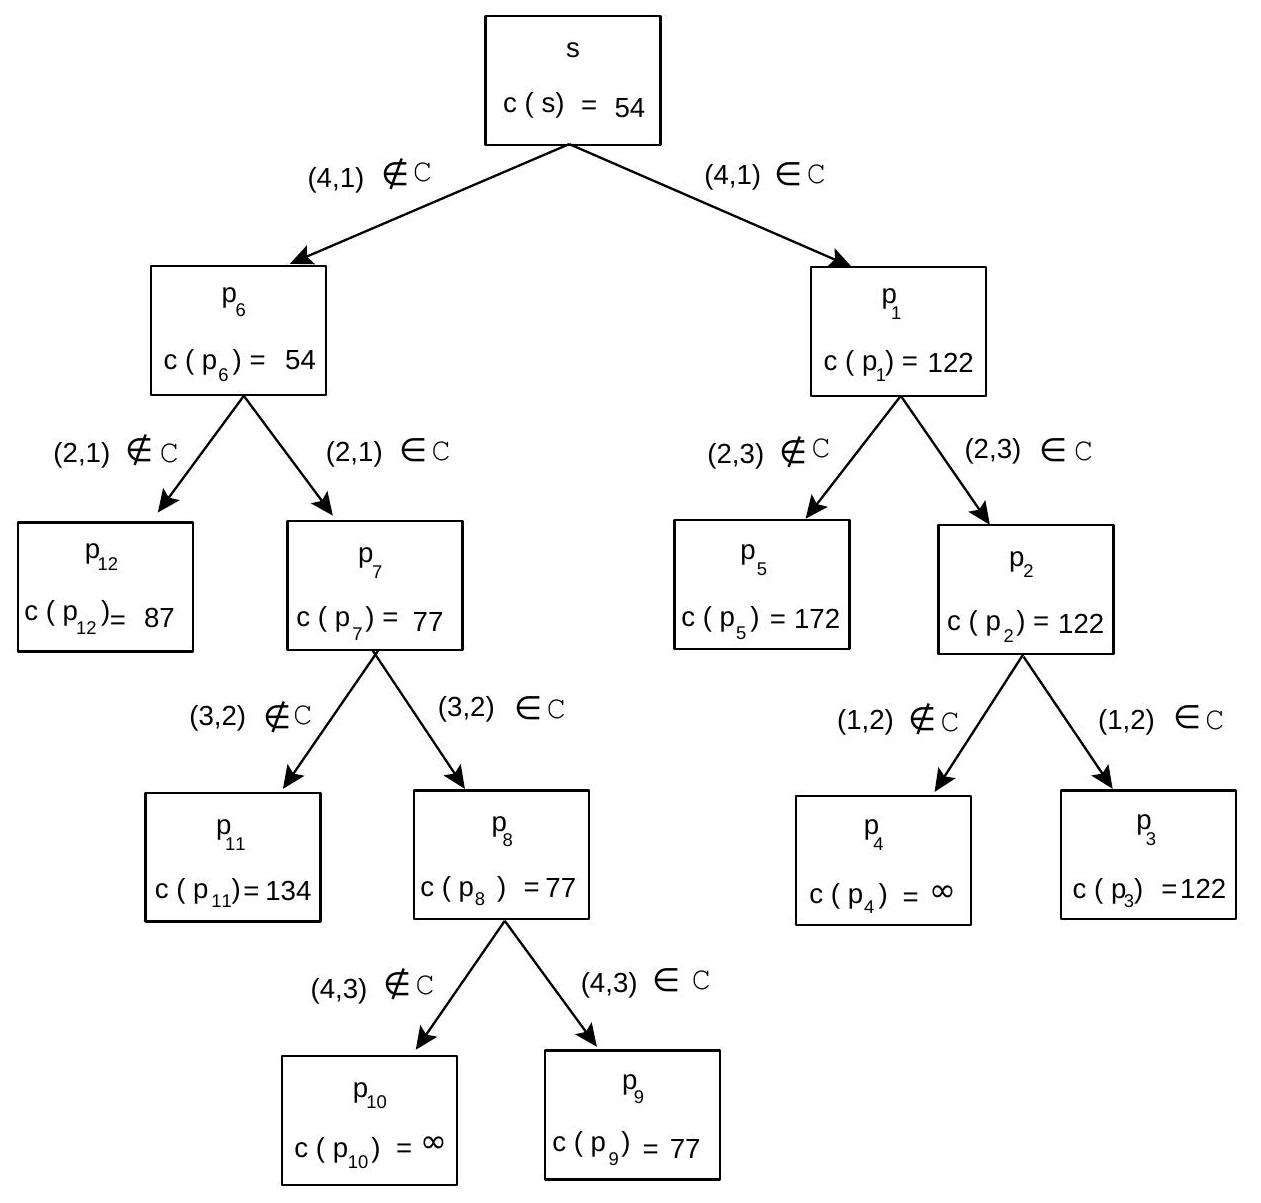
\includegraphics[max width=\textwidth, center]{2025_09_05_458e5b1ce89abceb5d44g-35}


\end{document}